\begin{filecontents}{localrefs.bib}

@report{GaloisPeter,
	author = {Peter Smith},
	title = {The Galois Connection Between Syntax and Semantics},
	journal = {Technical Report},
	publisher = {University of Cambridge},
	year = {2010}
}
@InCollection{SEP21,
	author       =	{Shapiro, Stewart and Kouri Kissel, Teresa},
	title        =	{{Classical Logic}},
	booktitle    =	{The {Stanford} Encyclopedia of Philosophy},
	editor       =	{Edward N. Zalta},
	howpublished =	{\url{https://plato.stanford.edu/archives/spr2021/entries/logic-classical/}},
	year         =	{2021},
	edition      =	{{S}pring 2021},
	publisher    =	{Metaphysics Research Lab, Stanford University}
}

@article{SVic91,
	title = {Steven Vickers. Topology Via Logic. Cambridge Tracts in Theoretical Computer Science, No. 5. Cambridge University Press, Cambridge Etc. 1989, Xiii + 200 Pp},
	year = {1991},
	volume = {56},
	doi = {10.2307/2275086},
	pages = {1101--1102},
	journal = {Journal of Symbolic Logic},
	author = {P. T. Johnstone},
	number = {3}
}

@article{LMN13,
author = {Williamson, Timothy},
year = {2013},
month = {03},
pages = {},
title = {Logic, Metalogic and Neutrality},
volume = {79},
journal = {Erkenntnis},
doi = {10.1007/s10670-013-9474-z}
}

@book{BPT00,
  author    = {Anne Sjerp Troelstra and
               Helmut Schwichtenberg},
  title     = {Basic proof theory, Second Edition},
  series    = {Cambridge tracts in theoretical computer science},
  volume    = {43},
  publisher = {Cambridge University Press},
  year      = {2000},
  isbn      = {978-0-521-77911-1},
  timestamp = {Mon, 22 Jul 2019 16:40:55 +0200},
  biburl    = {https://dblp.org/rec/books/daglib/0001441.bib},
  bibsource = {dblp computer science bibliography, https://dblp.org}
}
@misc{GalLogic17,
      title={A Galois connection between classical and intuitionistic logics. I: Syntax}, 
      author={Sergey A. Melikhov},
      year={2017},
      eprint={1312.2575},
      archivePrefix={arXiv},
      primaryClass={math.LO}
}
@misc{topo19,
      title={A semantic hierarchy for intuitionistic logic}, 
      author={Guram Bezhanishvilia and Wesley H.Holliday},
      year={2019},
      series={Indagationes Mathematicae},
      volume  = {30/3},
      pages  = {403-469}
}

@misc{intuitSeman17,
      title={Mathematical semantics of intuitionistic logic}, 
      author={Sergey A. Melikhov},
      year={2017},
      eprint={1504.03380},
      archivePrefix={arXiv},
      primaryClass={math.LO}
}
@inproceedings{HFCA05,
author = {Chen, Yaohua and Yao, Yiyu},
year = {2005},
month = {09},
pages = {285- 292},
title = {Formal concept analysis based on hierarchical class analysis},
isbn = {0-7803-9136-5},
doi = {10.1109/COGINF.2005.1532643}
}
@article{ConstructClassical,
  author    = {Russell O'Connor},
  title     = {Classical mathematics for a constructive world},
  journal   = {Math. Struct. Comput. Sci.},
  volume    = {21},
  number    = {4},
  pages     = {861--882},
  year      = {2011},
  timestamp = {Wed, 01 Apr 2020 08:48:57 +0200},
  biburl    = {https://dblp.org/rec/journals/mscs/OConnor11.bib},
  bibsource = {dblp computer science bibliography, https://dblp.org}
}
\end{filecontents}

\documentclass[]{llncs}
%\documentclass[final]{ieee}
%\usepackage{tikz}
%\include{zl-defs}
%\usepackage {latexsym,epsf,floatflt,pstricks}
%\usepackage{semantic, inference}
%\usepackage[table]{xcolor}

\usepackage[table]{xcolor}
%\usepackage{times,pstricks} 
\usepackage{tikz-cd} 
\usepackage {pst-node}
\usepackage {latexsym}
\usepackage{hyperref}
%\usepackage{amsmath,amscdx}
\usepackage[all]{xy}
\usepackage{mathpartir}
\usepackage {stmaryrd}
\usepackage {amsmath,cancel}
\usepackage {amssymb}
\usepackage {floatflt}
\usepackage{tikzit}
\usepackage{bussProof}
%\usepackage{standalone} Fails - might be use of filecontents for bibrefs
%\input{simple.tikzstyles}
\usepackage{hyperref}
%\setlength{\tabcolsep}{12pt}
\newcommand {\blank}[0]{\ensuremath{\_ }}
\newcommand {\eg}[0]{e.g.}
\newcommand {\ie}[0]{i.e.}
\newcommand{\DofD}{{\bf DofD }}
\newcommand {\setN}[0]{\ensuremath{\mathbb N}}
\newcommand {\AbsLH}[2]{\, _{#1}{Abs}_{#2}}
\newcommand{\s}[0]{\hspace*{1mm}}
\newcommand{\sa}[1]{\s #1 \s}
\newcommand{\shl}{ \cellcolor[HTML]{D0D0D0} }
\newcommand{\shd}{ \cellcolor[HTML]{A0A0A0}}
\newcommand{\shll}{ \cellcolor[HTML]{E0E0E0}}
\newcommand {\parp} [1]{ \hspace*{-0.5ex}||_{#1} \hspace*{-0.5ex}}
\newsavebox{\mybx}  
\newsavebox{\mybxx}  
\newsavebox{\mybxxx}  
\newcommand {\mythin}[4]
   {
\savebox{\mybx}{#1}  
\settowidth{\dslen}{\usebox{\mybx}}     
\addtolength{\dslen}{#4}
\begin{floatingfigure}[r]{\dslen}
\hspace*{#4}\hspace*{-1ex}\usebox{\mybx}
\caption{#2}   
 \label{#3}
\end{floatingfigure} 
   }
%\newsavebox{\mybx}  
\newcommand {\myfloat}[3]
   {
\savebox{\mybx}{#1}  
\settowidth{\dslen}{\usebox{\mybx}}     
\begin{floatingfigure}[r]{\dslen}
\noindent
\usebox{\mybx} \vspace{-3ex}
 \caption{\ #2}   
 \label{#3}
\end{floatingfigure} 
   }
\newcommand {\oldfloat}[3]
   {
\savebox{\mybx}{#1}  
\settowidth{\dslen}{\usebox{\mybx}}     
\begin{floatingfigure}[r]{\dslen}
\noindent

\usebox{\mybx}
 \caption{\ #2}   
 \label{#3 }
\end{floatingfigure} 
   }
\newcommand {\myfloatwo}[2]
   {
\savebox{\mybx}{#1}  
\settowidth{\dslen}{\usebox{\mybx}}     
\begin{floatingfigure}[r]{\dslen}
\noindent
\usebox{\mybx}
 \label{#2}
\end{floatingfigure} 
   }

\newcommand {\myfig}[3]
   {
\savebox{\mybx}{#1} 
   \settowidth{\dslen}{\usebox{\mybx}}
  \begin{figure}[!htb]
  \begin{center}
    \begin {minipage}{\dslen}{#1}\end{minipage}
    \caption{\ #2}
\label{#3}
  \end{center}
  \end{figure}
    }
\newcommand {\myfigtwo}[4]
   {
\savebox{\mybx}{#1} 
   \settowidth{\dslen}{\usebox{\mybx}}
  \begin{figure}[!htb]
  \begin{center}
    %\fbox{
   \begin {minipage}{\dslen}{#1}\end{minipage}
   %}
\savebox{\mybx}{#4} 
   \settowidth{\dslen}{\usebox{\mybx}}
      %\fbox{
    \begin {minipage}{\dslen}{#4}\end{minipage}
     %}
  \caption{\ #2} 
\label{#3}
  \end{center}
  \end{figure}
   }
\newcommand {\myfigf}[4]
   {
\savebox{\mybx}{#1} 
   \settowidth{\dslen}{\usebox{\mybx}}
  \begin{figure}[!htb]
  \begin{center}
    \begin {minipage}{\dslen}{#1}

   \footnotesize{#4}\end{minipage}
     \caption{\ #2}
\label{#3}
  \end{center}

  \end{figure}
   }

\newcommand {\myfigb}[3]
   {
\savebox{\mybx}{#1}  
\settowidth{\dslen}{\usebox{\mybx}}     
\noindent
\begin{figure}[b]
\noindent
\begin{center}
\makebox[\dslen][c] {
\usebox{\mybx}}  \caption{#2}   
 \label{#3}
\end{center}
\end{figure} 
   }

\newcommand {\Arop} [4] 
{\ensuremath{{#1}{{\stackrel{#2}{\Longrightarrow}}_{#4}}{#3} }}

%%%%%%%%%%%%
% Z sequence-filter
\newcommand{\zfilter} [2] { {#1} \upharpoonright{#2}}

%\usepackage {ifthen}
%\usepackage [dvips] {graphics}
\newlength{\dslen}
\newlength{\dslena}
\newlength{\dslenb}
\newcommand {\overo} [1] {\widehat{#1}}


\newsavebox{\mytab}
\newcommand {\mybox} [1]
   {
\settowidth{\dslena}{#1}
 \raisebox{\dslena}{#1}
  }
\newcommand {\parsyn} [1] {\stackrel{\parallel}{\scriptstyle #1}}
%\newcommand {\parsyn} [1] {\parallel_{\vspace{1ex}\hspace{-1ex}\scriptstyle #1}}
\newcommand {\refadt} [0] {Ref_{s}}
\newcommand {\scol} [0] {;\hspace{-0.5em}}
\newcommand {\sfa} [0] {\sf{a}}
\newcommand {\sfb} [0] {\sf{b}}
\newcommand {\sfc} [0] {\sf{c}}
\newcommand {\citepa} [0] {\cite{Ros97,Mil89,BaW90,Hen88b}}
\newcommand {\hplu} [0] {\ensuremath{\widehat{+}}}
\newcommand {\hpar} [0] {\ensuremath{\widehat{\parallel_{S}}}}
\newcommand {\htau} [0] {\ensuremath{\widehat{\tau}}}
\newcommand {\hdelta} [0] {\ensuremath{\widehat{\delta}}}
\newcommand {\hseq} [0] {\ensuremath{\widehat{\hspace*{0.5ex}; }}}
\newcommand {\hcon} [0] {\ensuremath{\widehat{[\_]}}}

\newcommand {\notangle} [0] {\ensuremath{\hspace*{0.1em}\angle \hspace*{-0.8em}\diagdown}}

\newcommand {\leftproj} [1] {\stackrel{\scriptstyle \gets }{#1}}
\newcommand {\rightproj} [1] {\stackrel{\scriptstyle \to }{#1}}
\newcommand {\pretotal} [1] {\stackrel{\scriptstyle \heartsuit}{#1}}
\newcommand {\lifttotal} [1] {\stackrel{\scriptstyle \bullet}{#1}}
\newcommand {\lsemantics} [0] {\lbrack\mkern-3mu\lbrack}
\newcommand {\rsemantics}     [0] {\rbrack\mkern-3mu\rbrack}

\newcommand {\plcsp}[1] {\ensuremath{{\parallel \atop{\scriptscriptstyle #1}}}}

\newcommand {\parcsp}     [1] {\ensuremath{
\settowidth{\dslen}{/{#1}}
{\hspace{-\dslen} {\hspace{\dslen}{\sf VM}\parallel{\sf Rob}/{#1} \atop{\scriptscriptstyle #1}}}}}
\newcommand {\partwocsp}     [2] {\ensuremath{
\settowidth{\dslen}{{#2}}
{\hspace{-\dslen} {\hspace{\dslen}(\_\parallel\_)/{#2} \atop{\scriptscriptstyle #1}}} }}


\newcommand {\absto}[1] {\ensuremath{\stackrel{#1}{\Longrightarrow}} }
%\newcommand {\mylgc} [3] {\ensuremath{
%\settowidth{\dslen}{\mbox {${#1}$}}
%\settowidth{\dslena}{\mbox {${#2}$}}
%\ifthenelse{\dslen < \dslena}{\setlength{\dslena}{\dslen}}{}
%\parbox[t]{\dslen}{\underline{#1} {#2}}
%\settodepth{\dslena}{\mbox ${#3}$}
%\raisebox{\dslena}{${#3}$} }}

\newcommand {\mylogic} [3] {
\xymatrix@R=0pt@C=0pt@M=0pt{&{#1} \\
\ar@{-}[rr] &&\hspace{1.0ex}{#3}\hspace{1.0ex}\\
&{#2}}}

%\newcommand {\mylgcy} [3] {
%\settowidth{\dslen}{\mbox{#1}}
%\settowidth{\dslena}{\mbox{#2}}
%\ifthenelse{\dslen < \dslena}
%{\parbox[t]{\dslena}{\underline{\makebox[\dslena]{#1}} {#2}}}
%{\parbox[t]{\dslen}{\underline{#1} \makebox[\dslen]{#2}}}
%%\settodepth{\dslena}{\mbox {#3}}
%\raisebox{-1.0ex}{#3} }

%\newcommand {\mylgcyy} [5] {
%\settowidth{\dslen}{\mbox{#1}}
%\settowidth{\dslena}{\mbox{#2}}
%\settowidth{\dslenb}{\mbox{#4}}
%\ifthenelse{\dslen < \dslena}
%{\setlength{\dslen}{\dslena}}
%{}
%\ifthenelse{\dslen < \dslenb}
%{\setlength{\dslen}{\dslenb}}
%{}
%{\begin{minipage}[b]{\dslen}
%\parbox[t]{\dslen}{\underline{\makebox[\dslen]{#1}}
%\underline{\makebox[\dslen]{#2}}
%\raisebox{-1.0ex}{#3}} \\ \mbox{} \end{minipage}
%\\ \parbox[t]{\dslen}{#4}\raisebox{-1.0ex}{#5}}}

\newcommand {\ct} [1] {\stackrel{\scriptstyle \circ \hspace*{-0.2ex} \to  }{T_{#1}}}

%%%\newcommand {\arocel}[3] {\ensuremath{
%%%{#1}\buildrel {#2} \over {\circ \hspace*{-1.0ex} - \hspace*{-1.1ex} - \hspace*{-1.1ex} \to }{#3} }}

%%%\def\rightcircfill{$\mathsurround=0pt \circ \mkern-2.4mu
%%%\\cleaders\hbox{$\mkern-2mu \mathord- \mkern-2mu$}\hfill
%%%\\mkern-6mu \mathord\to $}

%%%\\newcommand {\arocel}[3] {\ensuremath{Dij%%%\\settowidth{\dslen}{\hbox {${#2}$\hspace{1ex}}}
%%%\{#1}\buildrel {#2} \over {\hbox to \dslen{\rightcircfill}}{#3} }}



\def\rightharpfill{$\mathsurround=0pt - \mkern-6mu
\cleaders\hbox{$\mkern-2mu \mathord- \mkern-2mu$}\hfill
\mkern-6mu \mathord\rightharpoondown$}

\def\Rightmapfill{$\mathsurround=0pt \models \mkern-6mu
\cleaders\hbox{$\mkern-2mu \mathord= \mkern-2mu$}\hfill
\mkern-6mu \mathord\Rightarrow$}

\def\Rightarrowfill{$\mathsurround=0pt \mathord= \mkern-6mu
\cleaders\hbox{$\mkern-2mu \mathord= \mkern-2mu$}\hfill
\mkern-6mu \mathord\Rightarrow$}

\newcommand {\AroL}[4] {\ensuremath{
\settowidth{\dslen}{\hbox {$\langle{#2},{#4}\rangle$}}
{#1}\buildrel \langle{#2},{#4}\rangle \over {\hbox to \dslen{\Rightarrowfill}}{#3} }}


\newcommand {\Aroel}[4] {\ensuremath{
\settowidth{\dslen}{\hbox {${#2}$}}
{#1}\buildrel {#2} \over {\hbox to \dslen{\Rightarrowfill}}_{#4}{#3} }}

\newcommand {\aro} [3]
{\ensuremath{{#1}{\stackrel{#2}{\longrightarrow}}{#3} }}
\newcommand {\raro} [3]
{\ensuremath{{#1}{\stackrel{#2}{\gets}}{#3} }}

\newcommand {\arotwo} [5]
{\ensuremath{{#1}{\stackrel{#2}{\longrightarrow}}{#3}{\stackrel{#4}{\longrightarrow}}{#5} }}

\newcommand {\aroeltwo}[5] {\ensuremath{
\settowidth{\dslen}{\hbox {${#2}$}}
\settowidth{\dslena}{\hbox {${#4}$}}
{{#1}\buildrel {#2\hspace{-0.5ex}} \over {\hbox to \dslen{\rightarrowfill}}{\hspace{-0.5ex}#3}\buildrel {#4\hspace{-0.5ex}} \over {\hbox to \dslena{\rightarrowfill}}{\hspace{-0.5ex}#5} }}}



\newcommand {\Aro} [3]
{\ensuremath{{#1}{\stackrel{#2}{\Longrightarrow}}{#3} }}

\newcommand {\aroleft} [3]
{\ensuremath{{#1}{\stackrel{#2}{\longleftarrow}}{#3} }}
\newcommand {\arew} [1] {\ensuremath{\stackrel{#1}{\leadsto}}}
\newcommand {\defeq}  {\ensuremath{ \hspace*{0.5em}
\stackrel{\mathrm{def}}{=} \hspace*{0.5em}} }

\newtheorem {mypdef}      {Definition}
\newtheorem {myplemma}     {Lemma} 
\newtheorem {myptheorem}  {Theorem}
\newtheorem {mypass}      {Assumption}
%\newtheorem {myprwa}      {Real World Assumption}
\newtheorem {mypprop}      {Proposition}
%\newtheorem {myptheorem} [mypdef] {Theorem}

\newcommand {\sref} [1] {Section~\ref{sec:#1}}
\newcommand {\aref} [1] {Assumption~\ref{ass:#1}}
\newcommand {\dref} [1] {Definition~\ref{def:#1}}
\newcommand {\propref} [1] {Property~\ref{prop:#1}}
\newcommand {\pref} [1] {Page~\pageref{page:#1}}
\newcommand {\lref} [1] {Lemma~\ref{lem:#1}}
\newcommand {\tref} [1] {Theorem~\ref{thm:#1}}
\newcommand {\fref} [1] {{\bf Fig.~\ref{fig:#1}}}
%\newcommand {\rwaref} [1] {Real World Assumption~\ref{rwa:#1}}

\newcommand {\myproof} {\noindent {\bf Proof\hspace{1em} }}
\newcommand {\mylend} {\noindent \ensuremath{\hfill\Box}}
\newcommand {\mydend} {\noindent \ensuremath{\hfill{\Box}}}
\newcounter{lno}
\newcounter{listno}
\newcommand {\pcm}
{\ensuremath{\vert\hspace{-0.3ex}\vert\hspace{-0.3ex}\vert} }
\newcommand {\myprog} [1]
   {\begin{verbatim} \include {#1} \end{verbatim} }
\newcommand {\aroelp}[4] {\ensuremath{
\settowidth{\dslen}{\hbox {${#2}\hspace{0.5em}$}}
{#1}\buildrel {#2} \over {\hbox to \dslen{\rightarrowfill}}_{#4}{#3} }}

\newcommand {\harp}[3] {\ensuremath{
\settowidth{\dslen}{\hbox {${#2}\hspace{0.5em}$}}
{#1}\buildrel {#2} \over {\hbox to \dslen{\rightharpfill}}{#3} }}


\newcommand {\saroelp}[4] {\ensuremath{\scriptstyle{
\settowidth{\dslen}{\hbox {${#2}$\hspace{-0.5em}}}
{#1}\buildrel {#2} \over {\hbox to \dslen{\rightarrowfill}}_{#4}{#3} }}}
\newcommand {\aroelps}[4] {\ensuremath{
\settowidth{\dslen}{\hbox {${#2}\hspace{-2.0em}$}}
{#1}\buildrel {#2} \over {\hbox to \dslen{\rightarrowfill}}_{#4}{#3} }}

\newcommand {\aroel}[3] {\ensuremath{
\settowidth{\dslen}{\hbox {${#2}$}}
{#1}\buildrel {#2\hspace{-0.5ex}} \over {\hbox to \dslen{\rightarrowfill}}{\hspace{-0.5ex}#3} }}
\newcommand {\arop}
[4]{\ensuremath{{#1}{\stackrel{#2}{\longrightarrow}_{#4}}{#3} }}

\newcommand {\notaro}
[3]{\ensuremath{{#1}{\stackrel{#2}{\,\,\not\!\!\longrightarrow}}{#3} }}
\newcommand {\notarop}
[4]{\ensuremath{{#1}{\stackrel{#2}{\,\,\not\!\!\longrightarrow}_{#4}}{#3 }
}}
\newcommand {\compress} {\setlength{\itemsep}{0cm}
\setlength{\parsep}{0cm}
\setlength{\topsep}{0cm}}
\newcommand {\Obsmath}[0]{\ensuremath{\mathbb O}}

\usepackage {calc} 
\newcounter{hours}\newcounter{mins}
\newcommand{\printtime}{%
   \setcounter{hours}{\time/60}%
   \setcounter{mins}{\time-\value{hours}*60}%
   \today \hspace{1ex}\thehours:\themins }


\catcode`\@=11
\newdimen\cdsep
\cdsep=3em



\def\cdstrut{\vrule height .6\cdsep width 0pt depth .4\cdsep}
\def\@cdstrut{{\advance\cdsep by 2em\cdstrut}}

\def\arrow#1#2{
  \ifx d#1
    \llap{$\scriptstyle#2$}\left\downarrow\cdstrut\right.\@cdstrut\fi
  \ifx u#1
    \llap{$\scriptstyle#2$}\left\uparrow\cdstrut\right.\@cdstrut\fi
  \ifx r#1
    \mathop{\hbox to \cdsep{\rightarrowfill}}\limits^{#2}\fi
  \ifx l#1
    \mathop{\hbox to \cdsep{\leftarrowfill}}\limits^{#2}\fi
}
\catcode`\@=12

\pagestyle{plain}
\begin{document}
\title{Julia  IDE VSCode + Jupyter}
\author{}

\institute{
      \email{davidistreader@gmail.com}\\
      %\printtime
      }

% (78*(11/28)) *(113*(11/28)) +(12*(62*(11/28)))= 1652.60
% (78*(11/27)) *(113*(11/27)) +(12*(62*(11/27)))= 1766.06
% 
\maketitle
\thispagestyle{empty}

%%%%%%%%%%%
\vspace{-.5cm}
\begin{abstract}   
 The Julia Jupyter link is good for demos but lack the IDE so useful for program development hence the move to VSCode.
 
 
\end{abstract}

\section{Setting up Julia in VSCode}

Start VSCode then install Julia via VSCode. Julia in VSCode is easy to set up so that it only partially functions. The following recipe works - not sure why!
\begin{enumerate}
\item Open new empty folder.
\item Create an environment - From command pallet start Julia REPL
\item REPL \verb|pwd()| , \verb|cd("/Users/dstr/Documents/GitHub")| but ls is  \verb|readdir()|
\item in REPL(in VSCode): in the repl type "]" to enter the package manger
   \begin{enumerate}
      \item $Pkg>${\bf activate .}  activate current directory?
      \item $Pkg>${\bf add Plots, Statistics}    add packages of interest
      
   \end{enumerate}
   \item to run a program from within the julia REPL \verb|julia> include("Editor.jl")|
   \item In VSCode to find Julia source for methods from loaded packages: First click on Julia icon in left hand list, Then under the Documentation option type the name of the method in the search bar
 \item {\bf link the newly created environment to the editor} by clicking on \emph{Julia 1.7} in the status bar at the very bottom of the VSCode screen and then selecting the environment from the drop down list.  
 \item the REPL will appear in the task list bottom right of VSCode
 \item in the left edge of VSCode click on the Julia icon to see 
 \item To see plot or the results of BenchmarkTools  you must select "Execute active File in REPL"  in the drop down list at the top right of screen! And/Or  add readline() to end of file. But beware {\bf @benchmark ...} is run in parallel and may take a long time?
 \item it is trivial to save as a Local Git repository?
 
 \item  the Julia REPL that VSCode spawns will appear both in VSCode and in a new terminal outside VSCode. 
 
\item in the \verb|Julia> pwd()| works as shell pwd similarly \verb|Julia> run(`ls -l`)|  To change from {\bf julia$>$} to {\bf shell$>$} type {\bf ;} and to get back {\bf $\tilde{ }$ C}

\item to run shell commands in the Julia REPL try  \verb|readlines(`ls`)| or \newline \verb|split(read(`sh -c 'echo *'`, String))|  ! Similarly: \newline
\verb|run(`bash -c 'source $HOME/mybash_file ; blockMesh -help'`)|
\end{enumerate}

\subsection{Some basic navigation tips}
In terminal type {\bf $>$ jupyter notebook}  and set the kernal to Julia. Julia uses $<tab>$ completion within the notebook. Jupiter $<esc>l$  to show line numbers

Julia  package management Pkg:  is a repl with in the  Juila repl {\bf julia$>$}
Note using Julia within Jupyter is very slightly different from using the Julia REPL.

 \begin{description}
 \item[julia$>$] sin($\pi$)
 
 \item[julia$>$] @edit sin(1)  \#to go to the Julia implementation of sin OR in Jupyter {\bf ?sin}
 \item[julia$>$] import Pkg
 \item[julia$>$] ]   \# enter the package REPL
 \item [pkg$>$] activate  myEnv
 \item [pkg$>$]  add Flux PyPlot Plots
 \item [pkg$>$]  status \# to inspect the environment myEnv
 \item [pkg$>$]  \emph{\textasciicircum C} to return to {\bf julia$>$}
\end{description} 

\begin{description}

\item[Package contents] \emph{$julia>$using Flux} for a list of package contents type:

 \emph{$julia>$Flux.$<tab>$} for dropdown list of functions OR for output to screen
 \emph{$julia>$Flux.$<tab><tab>$} OR
 \emph{$julia>$names(Flux)} for function you should use.
 \item[Source code] from links displayed by:
 \begin{enumerate}
 \item \emph{$julia>$methods  fun}  will show the list of all  implementations
 \item \emph{$julia>$methods  fun(2,3.5)}  implementation with these parameters
  \end{enumerate}
 \item [help] \emph{$julia>$?} to enter the help system.
 
 \emph{$help?>$gradient}  will then list details of the gradient function and exit the help system.
 
 \item [methodswith Type]   \emph{$julia>$ methodswith(DataFrame)}  for list of methods that apply to objects of type \emph{DataFrame}
 \item [Search Git Hub]  \href{https://juliahub.com/ui/Search?q=&type=packages&t=function&u=define} {Julia Search!} fantastic
 
\item [cheat sheets] 1) \href{https://juliadocs.github.io/Julia-Cheat-Sheet/} {Julia-Cheat-Sheet}
and 2) \href{https://cheatsheets.quantecon.org/} {Matlab-Python-Julia}
 
 
 \item [Your function documentation] that will show up in jupyter with \emph{$>$?cont\_game}:
 \begin{verbatim}
"""
 cont_game(`\delta`, P) 
- `\delta` small x inc
- `P` prob  
``P = \delta^n``
"""
function cont_game(\delta, P) 
    return P
end
\end{verbatim}
\end{description}
 
 \subsection{Julia Efficiency}
 Julia is JIT compiled, thereby  defining functions with UNtyped parameters can  provide extreme Modularity of package construction without loss of efficiency. It also means that a function is compiled once for each time it is called with parameters of distinct type thus allowing code optimization over function boundaries. Thus the use of {\bf Val} type parameters makes the value available to the compiler and allows additional efficiency via compile time code optimization.
 \begin{enumerate}
 \item define function with additional parameters over use of global variables
 \item break functions into separate functions over conditions on type
 \item use inplace updates over allocation of heap variable 
 \item avoid untyped collections use subtyping {\bf \{T<:AbstractFloat\}}
 \item declare variables as {\bf const} where applicable
 \item to check efficiency us {\bf @time, @allocated, @profile} or {\bf using Traceur}
 \end{enumerate}
 
 \subsection{Julia Idioms}
 
 try macros @code\_warntype, @code\_llvm, @time 
 
 Vectors can be reshaped into a matrix - avoid computing in global scope, always use functions to do the commutation global variable declared const are efficient.
 
 Defining your own type can be very efficient - look up \emph{type instability}. Julia encourages not using explicit types to allow library modularity and the compiler uses \verb|Base.convert| to perform type conversion. 
 
 Defining your own struct/type is common and produces something immutable. You can add your own \emph{inner constructor} - say  to prevent negative values being used. 
 In julia you cannot redefine a type: \verb|>workspace()| removes previously defined types.
 
 Parametric types have poor type inference hence require explicit typing of parameters \verb|foo{Int}(3)|,  but you can code this in the inner constructor to be able to type \verb|foo(3)|.
 
 To define a method for \verb|+| on your struct first \verb|import Base.+| and then define the metod that will be added to the \verb|Base|.  See \verb|Base.promote_type| and \verb|Base.promote_rule|.
 
 Pretty printing your struct can be done by overloading \verb|Base.show| and converting its type can be used by overloading \verb|Base.convert|.
 

 
\subsection{Julia Metaprogramming}
Used to construct a \emph{Domain Specific Languages}, DSL and to build repetitive code. But, frequently higher order function are preferable.


Julias MetaProgramming is Lisp like and provides functions with code in, data of type \verb|Expr| and code out (note assignment is an \verb|Expr|.  The Julia  function  \verb|parse| converts Strings to Expr and \verb|eval| executes a Julia \verb|Expr|.
The \verb|Expr| are recursively defined trees and ou can use pattern matching  to detect the sub-expressions you wish to change. The Julia parser will accept some latex symbols but you need to define what they mean!
 
 
 Look up \verb|dump| and \verb|Meta.show_sexpr|
  Overflow is not always checked for and can be a problem. But, checking can be added using \verb|Base.checked_mul| \ldots. 
  
  With \verb|ex = :(x-1)| defines  \verb|ex::Expr|, note ex contains  a data structure, then     \verb|$ex| maps this data structure and returns  the function \verb|(x-1)|
  
To add assignmnets to an expression use \verb|Base.push!(ex.args, x=a)|  


Lookup Julia \verb|macro|,  \verb|Macro.quote|, \verb|macroexpand|  and {\bf Macro Hygiene} about variable in Global space.

 \section{Neural Nets}
  Neural nets can be very flexible as they are universal function  approximators. But, in machine learning in general,  flexibility has both pros and cons, it can result in more complex computation  - slow  training and  over-fitting. Some advances in neural nets come about by restricting their flexibility so that they more closely model the domain of interest.
  
 \subsection{A Neuron}
The $i$th neuron holds a hidden value $h_i$ with $j$ inputs and $k$ outputs has three  parameters that can be fixed or learnt during training:
\begin{center}\begin{minipage}{2in}
\begin{enumerate}
\item $W_{ij}$ the weight matrix
\item $b_i$ a scalar bias
\item $\rho_i$ an activation function
\end{enumerate}\end{minipage}\end{center}
The hidden value in the nodes were initially just scalar values but over time much more complex structures were used.

Beware much of the literature assumes that the activation function is less important and frequently  fixed both over time and over the whole net.  
  
  \subsection{Neural layers}
  A neural net is built from a  discrete collection of neural layers an input layer, an output layer and a collection of hidden layers, each layer is a discrete collection of neurons.
  
  Initially the inputs and outputs were vectors of scalar values but over time more complex data structures were used. Simple  Neural Nets can be viewed  as  parametrised algorithms that compute functions over some vector space such as $f:\cal{R}^n\rightarrow\cal{R}^m$, mapping pictures to categories. 
  
 Although the neural net can only output the value of the function at a discrete set of points where appropriate the value of the function between the points can, up to some margin of error, be computed by \emph{interpolation} and beyond the range of known values by \emph{extrapolation}. By these techniques the values of the neurons can be interpreted as parameters over some basis polynomials and Fourier series being common. 
 
Supervised learning requires pairs of input and output vectors. In the forward pass  data is input, from which  the value of the hidden layer is computed from this the output layer is computed. 
A

\vspace{1mm}\begin{center}\begin{minipage}{2in} 4.  loss function \end{minipage}\end{center}

\noindent is applied between the computed output and the known output vector. The backward pass adjusts the networks parameters with the goal of improving the next forward computation of the output vector.Supervised learning of neural nets uses training data consisting of input, output pairs of vectors and test data consisting of only input data. Supervised learning is most effective when the training and test data include the same features and have the same distribution. 

The meaning of the output values is defined by or is used to define the loss function of the network.

Where the amount of test data is to small \emph{transfer learning}, training on abundant data that is similar but not the same as the test data, has been know to increased effectiveness. 
 One way to explain the effectiveness of  transfer learning is that the training and test data   both share   a common abstract  model.
 
A shallow neural net SNN has  an input layer, an output layer and a single hidden layers.
Although each layer consists to a set of nodes for efficiency this may be implemented with an array but the order has, in general, no semantics.
 
 Universal function approximation: for SNN with one of many simplifications a. with bounded weights, b. with fixed activation function. Initially this led to not considering Deep NN



\subsection{Deep Neural network} consist of an input layer, an output layer and a stack of several hidden layers.  With the addition of each layer there is an expansion of the number of parameters. Normally in machine learning this increase in the number of parameters would result in errors due to \emph{over fitting} but this rarely happens in DNNs. 


Other than for the input layer each $j-$neuron has a weight attached to each $i-$input $W_{ij}$, a scalar bias $b_j$ value and an activation function $\rho_j$ .
In the  forward pass the input values  are multiplied by the weight, the results are summed along with a bias  $r_j=\Sigma_{i=1}^{i=n} x_i*W_{ij} + b_j$ . This is input to an activation function prior to the result $\rho_j(r_j)$  being output. 

For some neural algorithms the activation function is of little significance and can be decided after the the rest of the neural architecture has been fixed. But for other algorithms the selection of the activation function is critical and must be designed along with the rest of the neural architecture.
Using appropriate activation functions a NN can be used to compute multiplication and division as well as summation. This enables the NN to to compute many  finite element methods, FEM.
 Further the activation function can be parametrised per neuron or per layer and learnt just like the weights and biases. This has been used in XPINNs.  Adaptive activation functions is equivalent to second order approximation bt without computing the Hessian, which is expensive.




The basic Multi Layered Positron,MLP, consists of a sequence of layers with total connection weight matrix between any two adjacent layers. 


Although given a large enough MLP and function can be modelled in practice MLPs were of little use until the physics of the problem at hand was embedded in the NN. A MLP can be thought of as having an unstructured topology whereas many more effective NNs have a physics inspired topology.



Convolution NNs were used for image recognition. The Topology of the layers captured: neighbouring neurons-pixels are more relevant than distant pixels; a feature, face, is a face wherever it appears and at whatever scale. Recurrent Neural Nets, RNNs,sequentially process data such as text by using the understanding of the initial part of the sentence when interpreting later words. Long Short Term Memory NNs, LSTM, are an improvement on RNNs. 
Attention Neural Networks are more flexible than RNNs as they process each word in parallel and also allow words at the end of the sentence to influence the interpretation of words appearing earlier in the sentence.

 Neural Net Architectures are often best described as the composition of collection of component  blocks of neural nets. Hierarchical Neural Nets capture abstract and more concrete understanding. 
 
 
 Attention Neural Nets mimic the flexibility of cognitive attention. They have three components an encoder and a decoder with an attention unit between them.
Transformer Neural Nets, like RNNs and LSTMs process sequential data but unlike RNNs and LSTMs they process the data in parallel using attention to select the relevance of the data.





{\bf Solving Inverse Problems with Deep Learning} by Lexing Ying

{\bf When and why physics-informed neural networks fail to train} by Paris Perdikaris looks at when and why failure occurs.

\subsection{Complex Valued NN}
Although the flexibility of NN can be greatly beneficial it can also be the cause of problems
Using Complex values in place of real values can limit this flexibility, preventing infeasible solutions from being considered and reducing over fitting. See {\bf A Survey of Complex-Valued Neural Networks}. CVNN are not the same a a two dimensional real NN but are good fro modelling data as amplitude, phase pairs.
  
\section{Linear Transformations}
Physical systems often have many parameters, many independent variables and many independent variables. When these are real scalar values the system is defined by a function from $n$-dimensional space to $m$-dimensional space. Even when you have a function defining a system its behaviour can be very hard to understand.

  Restricting ourself to  very simple functions, transformations, both helps and is of practical usefulness. linear transformations:
  \begin{enumerate}
  \item preserve the origin  $f(0) = 0$
  \item keep the axies parallel   $f(x+y) = f(x) + f(y)$
  \item preserve relative distance. $f(nx) = nf(x)$
  \end{enumerate}
 
 Each element of the space is given by a vector over some basis. Any Linear Transformation is 
 defined by a Matrix. Each column of the matrix defines what a unit of the basis is mapped to. The effect of the Linear Transformation $lt$ is given by the multiplication of its Matrix representation $M_{lt}$ with    a vector in the input basis $lt(\overrightarrow{v}) = M_{lt}\overrightarrow{v}$.
 
  The determinant of the Matrix defines the volume of the paralelapiped that the unit hypercube is mapped into. \emph{Is this a special case of  the {\bf divergence} of  a non-linear transformation?}
  
  \section{Differential Equations}
Many physical systems can  can be more easily defined in terms of the rate of change in the system than in terms of the value of the system. We let simple systems have one independent variable, input, and one dependent variable, output the value of the system can be visualised by the graph of a function $u(t)$ and the rate of change as the gradient or derivative of this function $u'(t)$.  The \emph{critical points} of a function are those where the gradient is zero, these prove very important as they capture many interesting features of the system including fixed point behaviour.
  
  {\bf Scalar system}s have  multiple independent variables $u(x,y)$ and a single scalar dependent variables the function can be visualised as an $n$ dimensional  surface. The gradient of a surface is a vector
\[\Delta u(x,y)  = \big[\frac{\delta u}{\delta x},\frac{\delta u}{\delta y}\big] \]

With multiple independent variables and multiple dependent variables the system maps spaces to spaces and can be represented as  a vector of scalar functions:
\[ u(x,y) = \big[ u_1(x,y), u_2(x,y)\big] \]
The gradient of $u$ is given by the Jacobian matrix.


The second order derivative of a scalar system $u(x,y)$  is the Hessian or derivative of the gradient and thus 
the Hessian is the Jacobian of the derivative.



  
  
\section{Scientific machine learning}
In this setting the many of the models are functions of both time $t$ and space $x$ that in addition are parametrised $p$. Thus the function to be learnt $u(t,x,p)$  may be very  complex and may be partially understood.


\subsection{Finite Element Methods}
FEM solves problems over N dimensional continuous domain by applying a discrete mesh over the  domain, solving for the points on the mesh and interpolating between the points. The accuracy of many methods can be improved by adjusting the mesh to concentrate on specific regions, \emph{r-adaptivity} or by increasing the the number of points in specific regions \emph{h-adaptivity}.

\subsection{NN-FEM}

Over many years efficient algorithms have been designed to find the solution to complex PDEs,..  Even when such algorithms exist neural nets can prove useful as much of the computation is moved to the training and allows near instance lookup of results for new inputs.

  Encoding the mesh points as the bias on the input layer means that training will automatically adjust the mesh to the desired regions , automatic r-adaptivity. Mesh points are Neurons and are elements in an array hence mesh points can be added at locations where they are most needed simply by adding elements to the array. This is h-adaptivity. With FEM-NN rh-adaptivity is learnt not designed by hand.

\subsection{Co-ordinate Discovery}
Autoencoder are used for coordinate discovery (Principle component analysis,  POD,..) in its simplest form a deep dense feed forward network with small dimensional middle layer. Train to minimize the difference between the input and output. Hence middle layer is a low dimension coordinate system.

\subsection{Sparse Identification of Non-linear Dynamics, SINDy}
Use a library of $n$th order terms, polynomials, trig functions, .. Train to find parameters to minimise $In-\Sigma_i t_i*P_i$ where $In$ is input. By adding to the loss function a penalty depending on the size of the non-zero parameters will encourage sparsity. Truncation of $p_i< \epsilon$ helps. (first order OR second order?)

SINDy has been successfully  used in conjunction with coordinate discovery. Some Afine transformation may be required to see the result is the same as the known input.


\subsection{Physic Informed Neural Nets, PINNs}

The integration of Physics and Neural networks has proven very effective.Physics can be encoded within Neural Networks in the:
\begin{description}
\item [Topology of the network]  such as CNN and Recurrent NN
\item [the Loss function]  such as PINN. Using automatic differentiation we  can evaluate the model represented by an ODE. Hence the Loss function includes not only $L_D$ the difference between the NN computed value and the training data but also $L_R$, the difference between the NN computed value and the value computed by the ODE.
\item [the activation functions] encoding laws in fixed or learnt activation functions
\item [by generating training data] $L_R$ can be used in place of $L_D$, if you have the data that is good if not you can always fake it.
\end{description}





\subsection{Hierarchical Neural Nets} HiDeNN adopts a flexible block structure that is intended to cover a range of existing architectures.

\begin{center}
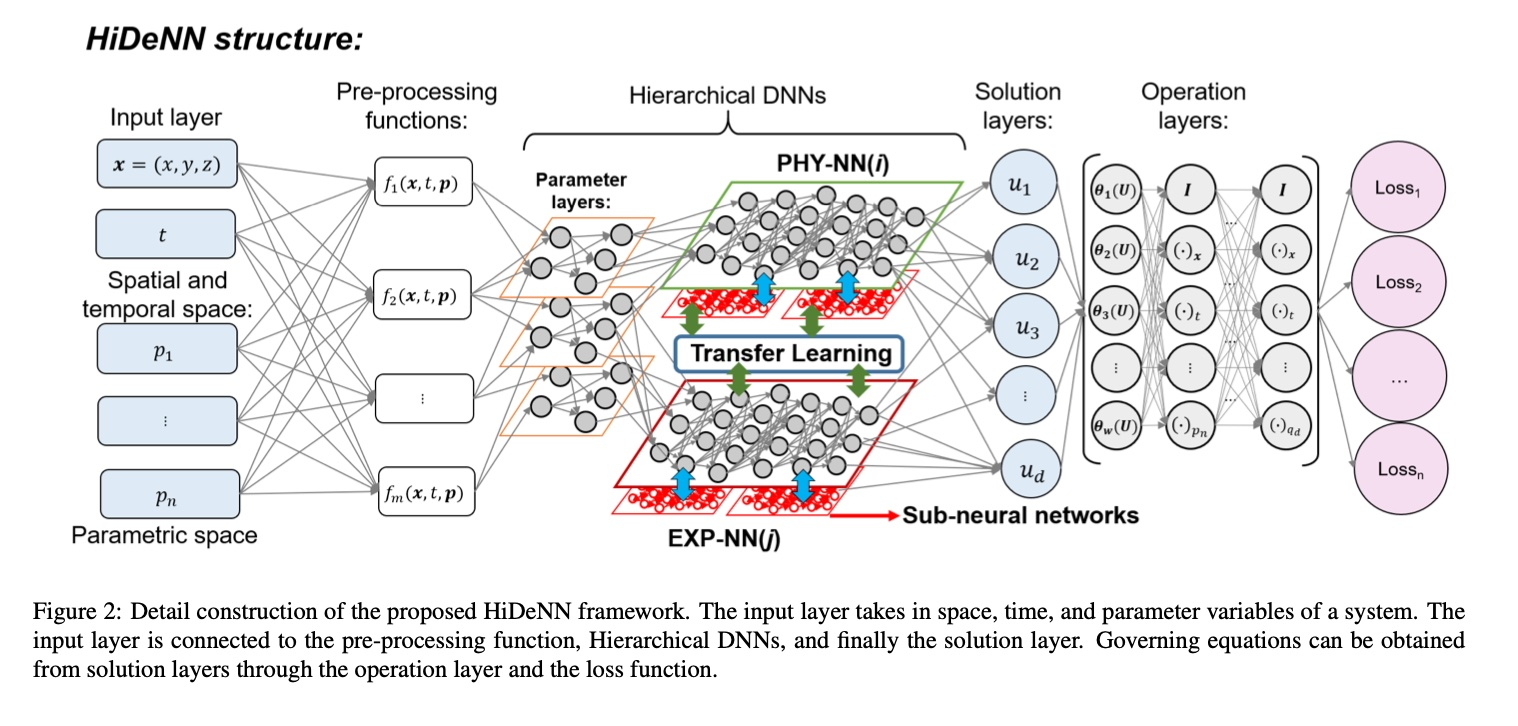
\includegraphics[width=100mm]{HiDeNN.jpg}
\end{center}

\subsection{Operator Neural Nets}
Normally the inputs and outputs  are vectors of scalars. Replacing these vectors with functions  we have an operators neural net, {\bf ONN}. An operator could be differentiation, integration, an ODE, \ldots

On some defined functional coordinates, polynomials, Fourier series, approximate the function as a linear function and learn.

Spatial data as input apply a Fourier Transform prior to input to the NN then reverse Fourier transform to return to original coordinates. Has the advantage that multiplication of the transformed input is ...

\begin{center}
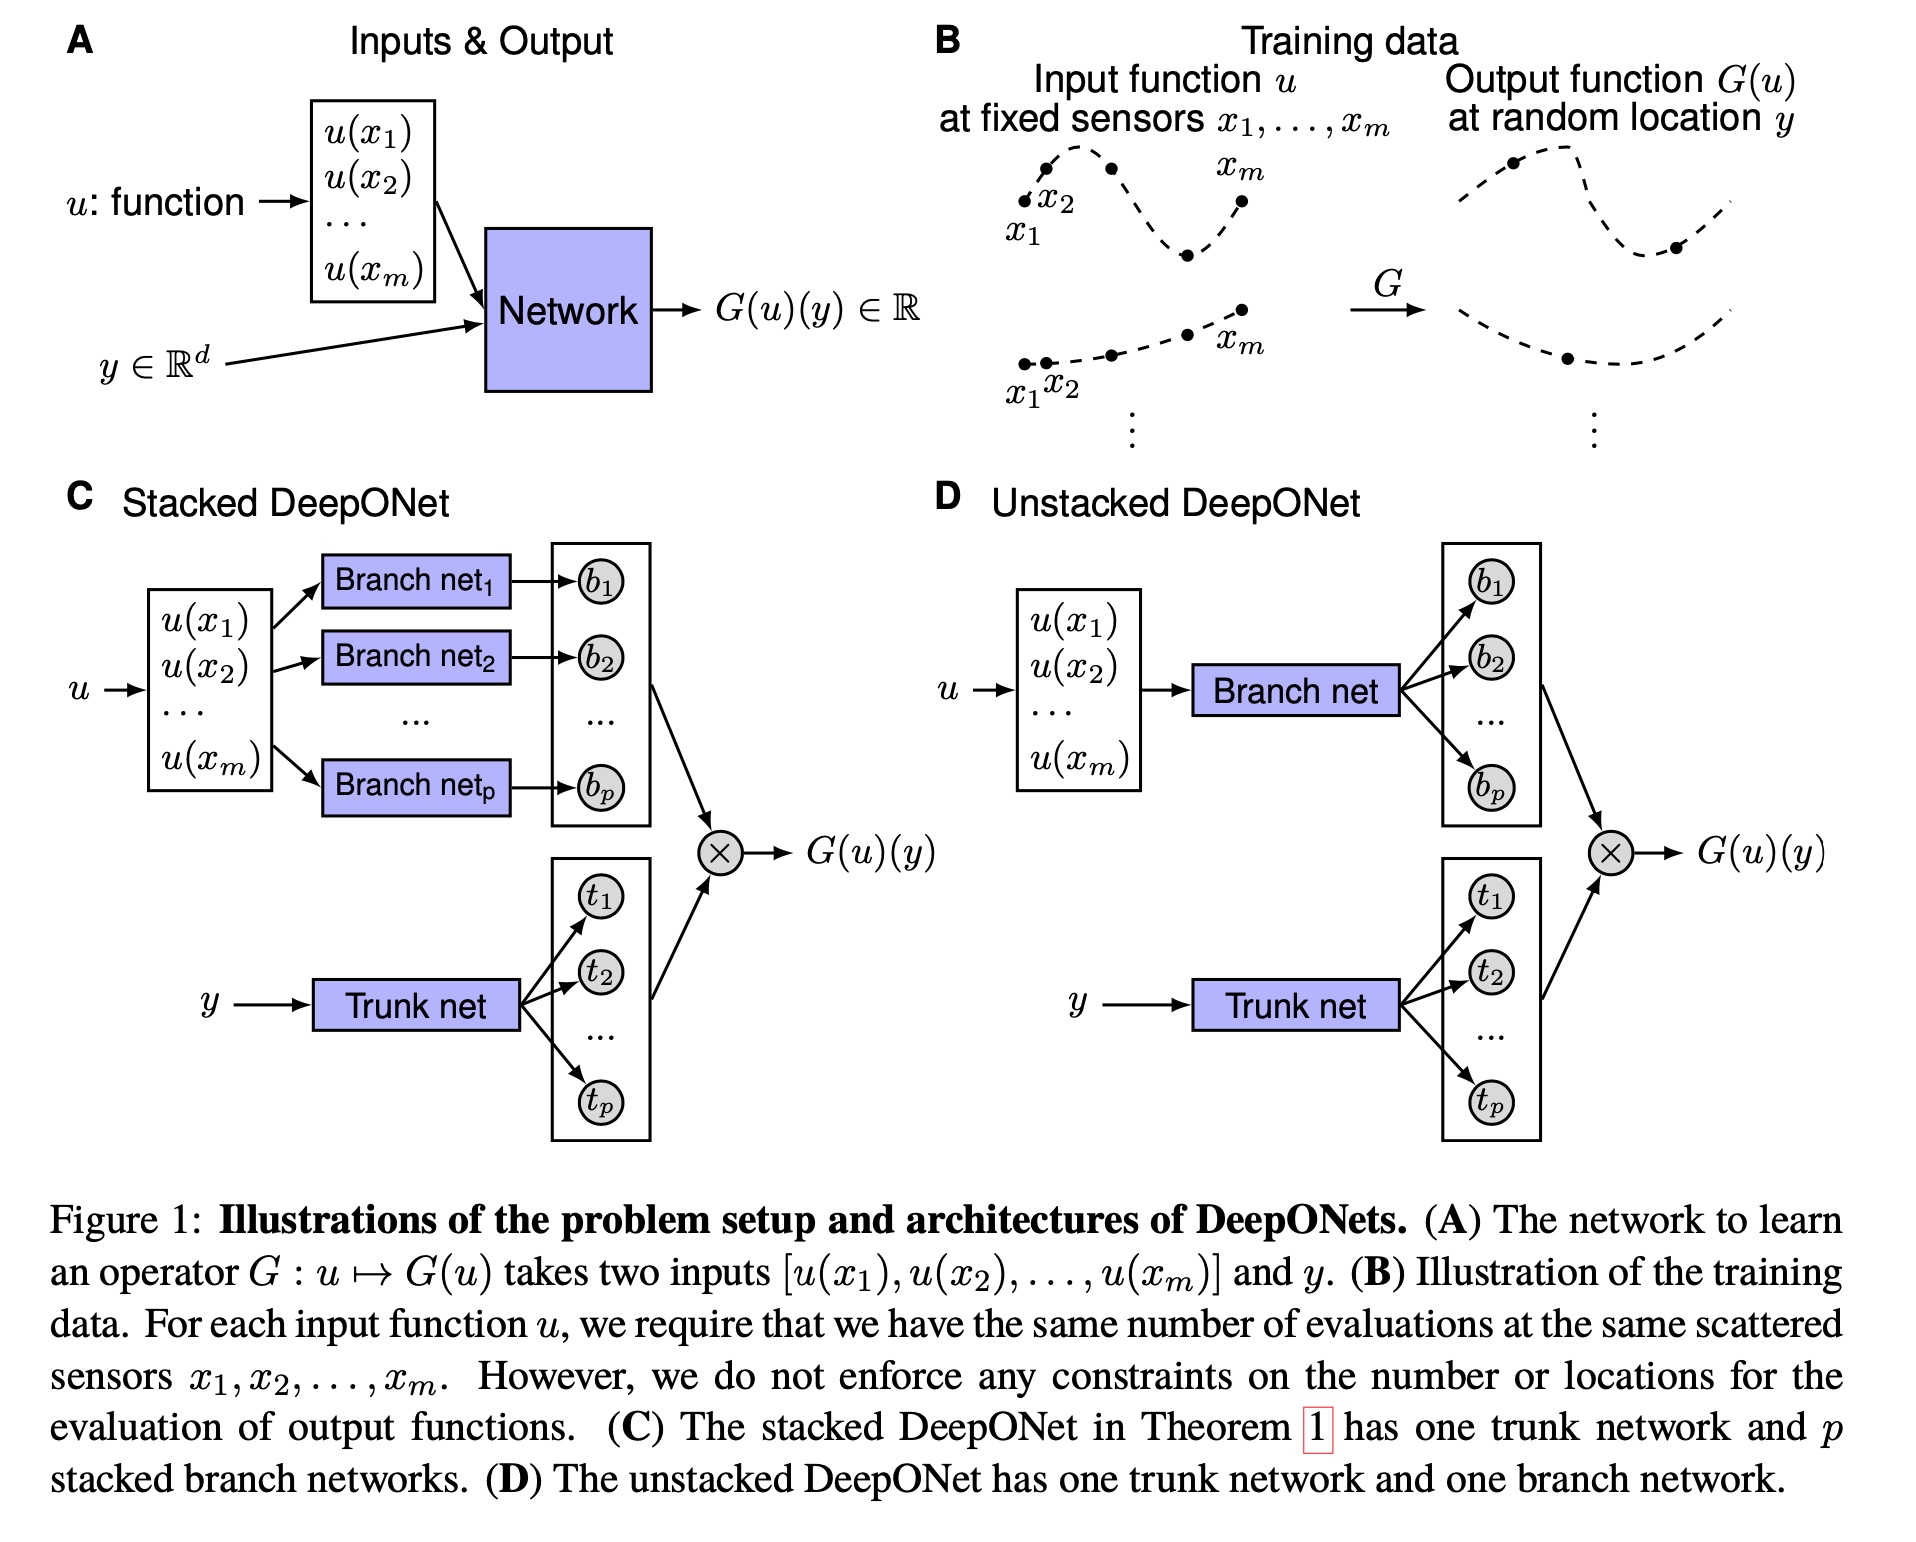
\includegraphics[width=100mm]{DeepONets.jpg}
\end{center}

\subsection{Message Passing Neural Nets}
Our starting point is \emph{Graph Neural Nets}, GNNs. Normally it is the hidden state of one neuron,$i$,  that is used  by another neuron $j$ to update its hidden state $h_i*w_{ik}$. The sending of messages disconnects the direct link between a nodes hidden state and its effect other neurons.


Graphs appear everywhere: chemicals, transport, brain function, mycelia function, etc. GNNs generalise CNNs.
\begin{enumerate}
\item  Antibiotic discovery
\item  Google maps directions
\item Pintrest
\end{enumerate}
An image can be seen as a regular square  Graph where the nodes are  pixels but, a pixel is a pixel wherever it appears. A sentence is a sequence, a linear graph, of tokens. 
Graphs generalise this by allowing: a. less regular structure and b. individual features on nodes, and c. the nodes have no fixed order unlike CNNs and RNs. 

MPNNs are built on GNNs and have an \emph{update phase} where, for T tie steps, the messages are used to update the node features, and/or edge features, and a \emph{readout phase} where the node features are aggregated to produce whole graph features. 

The MPNN will learn three functions 
\begin{enumerate}
\item M, how to aggregate Messages
\item U, how to update Node features
\item R, how to report Graph features
\end{enumerate}   
Allowing these function to be anything introduces extreme flexibility and they have been restricted in a vast array of ways in different approaches.





GAT graph attention networks.
Transformers as GNNs

Define parallel composition of GNNs of processes and learn solution?
? Symbolic Bisimulation ?

\subsection{Graph Feature analysis}
Graphs can have features both on nodes and on edges. What those features are can be designed by hand or learnt from the data.  Learning a mapping from nodes to an $n$ dimensional vector

\subsection{Graph Attention Neural Nets}
Initialise the Attention Matrix with  the Graph structure then learning the attention network becomes  \emph{learning the graph} structure.



\section{Organic Molecular Chemistry}
Chemicals are naturally represented as Chemical Graphs, CG, with atoms at the nodes and chemical bonds as edges.  SMILEs represents chemicals as strings.  Prediction of chemical properties have been recently been successfully predicted using MPNNs, both at the quantum level and the pharmacological level.

This area cries out for models at multiple levels of abstraction  -- baby dreaming!


Initial paper uses MPNNs to convert text description of chemicals,SMILEs, for the classification of the chemicals. They make use of standard text analysis NNs and  the resulting graph representation of the chemical seems to have little to do with the Chemical Graphs!

Open source \href{https://www.rdkit.org/} {RDkit} transforms SMILEs strings into chemical graphs.

Another source of data is the libraries of hand crafted chemical  descriptors


\subsection{Graph Neural Networks, GNN}
The graphs they consider include LTS and PN.  Loss functions for bisimulation appear to fit well with GNN. Extensions for the computation of equivalence between Continuous and Stochastic Petri Nets, CPN/SPN, seen very feasible.

SPN, with their use of rate function appear to have equivalent expressive power to ODEs and hence will be just as difficult to interpret. Different bridges between SPN and ODE are actively being used in the modelling of biological and chemical systems.


\subsection{Graph Attention Networks}



What are chemistry relevant questions? Or, rephrasing, what are the chemistry relevant features?
\begin{enumerate}
\item the Graph
\begin{enumerate}
\item bond strength at temp $\theta$ 
\item reaction rate  at temp $\theta$
\item vibration rate?
\item electron shell occupancy?
\end{enumerate}
\item the folding
\item the substructures
\end{enumerate}

What are the machine learning tools?


\section{Parallel Computing and Scientific Machine Learning} 
Many thanks for open source  MIT course $18.337J/6.338J:$ gores over how to build optimized libraries that can be used. So covers a lot of  underlying theory.
Scientific Machine Learning is the use of Machine Learning to the solution of the simulation of Scientific problems. Machine learning on data is simply this problem of finding an approximation to some unknown function!

Neural Nets, Talyor series and Fourier series are all universal function appropriators that can be used with loss function in standard parameter optimisation procedures. But Neural Nets  do not scale exponentially with the dimension of the input. In theory given enough data and a large enough neural net you can solve any problem. In practice it is necessary to encode as much of the behaviour of the system as you can into the neural net prior to training it, for example convolution neural nets. Many disciplines use differential equations to capture some of the behaviour of the systems they are modelling.

Differential equations describe the behaviour whereas neural nets learns the behaviour from the data. ODEs are better at extrapolation than neural nets and are interpretable.

Neural Ordinary Differential Equations  $u'(t) = f(u,p,t)$  where $f$ is a neural network.




Dynamic systems change over time and can be defined as a set of differential equations For example the N body problem is defined by N ordinary differential equations, ODEs, $F=MA$ where A - acceleration - is the second order differential of position over time. A solution to these differential equation is a function from time to position.

ODEs  are of the form $\frac{du}{dt} = f(u,p,t)$. When there is a vector  $u=(u_1,u_2,\ldots u_N)$ then $\frac{du}{dt}$ is the Jacobian. And the Jacobian, of such an ODE is defined in terms of partial derivatives. 

PDEs, Partial Differential Equations are a generalisation of ODEs that allow terms such as $\frac{\delta u_i}{dt}\frac{\delta u_j}{dt}$ etc.

ODEs can be solved, the explicit function $u(t)$ constructed, for a given vector of the parameters $p$. The solution is frequently best understood by plotting the result, $u(t)$ plot.  Another useful way to understand a dynamical system  is the bifurcation plot.

\subsection{Algebraic Dynamics}

{\bf AlgebraicDynamics.jl} provides a way to \emph{"wire"} together different models, eg: the flow of people between cities, each with their own SIR infection model.

\subsection{Latent Differential Equations}

{\bf LatentDiffEqu.jl} Encode high vector space input (video of pendulum)  into low dimension space (to 2) using RNNs or LSTMs  then decode back to high vector space output. Use SINDy to convert low dimension space into analytic term.

Physics-Informed ML Simulator for Wildfire Propagation

\subsection{Baysian Inference }

{\bf Turing.jl} allows Probabilistic programming. With {\bf Flux.jl} you have Neural ODE models.

\subsection{Physics Informed Neural Nets}

Machine learning is data driven and can use neural nets to model dynamic systems. These same dynamic systems can be analyticity modelled by differential equations. Physics Informed Neural Nets {\bf PINN} attempts to combine the best of both worlds:

\begin{description}
\item[NN] Robust to noise
\item[NN] Good with high dimensional input
\item [NN] Can infer hidden pattern, implicit basis
\item [ODE] fast to compute
\item [ODE] No input data needed
\item [ODE] Error bounds on solution
\end{description}

Automatic differentiation of NN used alonge with ODE encoded in Loss function.


Auto Encoder Decoder that relates  high dimensional  system, such as video input, to low dimension representation, such as pendulum dynamics of the single $\theta$ variable   representation can be learnt. Then $\theta' = f(\theta)$ dynamics  can be learnt.

\subsection{Automatic Differentiation}
Given a program the compiler constructs a \emph{primal},  an executable algorithm. Using {\bf Dual Numbers} the AD compiler  also construct an executable algorithm for the differentiation of the primal. 
\begin{description}
\item [Forward mode AD] asks the question: how dose the output change when the input changes by some small amount?  Forward Mode AD is efficient at computing the gradient when there is one, or a small number, of inputs but is terrible when there is a large number of inputs.
\item [Reverse Mode AD] asks the question the other way around. How should the the inputs be changed  in order to change the output by a small amount. Reverse Mode AD is efficient at computing the gradient when there is a large number of inputs.
\end{description} 
Forward  Mode AD is often compared with the forward pass of a neural net and Reverse Mode AD is compared with back propagation and clearly you cannot replace back propagation with a forward pass.
Forward and Reverse Mode AD both compute the gradient. But are they the same function or, ignoring efficiency, is Reverse Mode doing something the Forward Mode is not? Alternatively are there applications using Reverse Mode where, ignoring efficiency, Forward  Mode could not be used?

The reason for asking this is that the paper \href{https://richarde.dev/papers/2022/ad/higher-order-ad.pdf}{\bf Provably Correct, Asymptotically Efficient, Higher-Order
Reverse-Mode Automatic Differentiation} defines Reverse Mode AD as a correct and efficient way to compute the gradient when there is a large number of inputs. Yet this is computing the exact same thing as  Froward Mode AD.


\subsection{Lecture 2}
JIT compilation slows down first execution but allows modular development of libraries.
Multiple dispatch and being a high level language allows aggressive code optimisation. 


For Julia efficiency
\begin{enumerate}
\item only benchmark functions and always use functions
\item Avoid explicit typing - no  overhead, $\mathbb{O_C}$, with JIT compilation
\item a $@view x[i:j]$ is a pointer to part of an array
\item Avoid heap allocation - for small size data use static vectors  for large size arrays allocate  prior to iteration (use mutating functions) and be aware of index order as arrays are implemented as single index linear structures.

\item broadcast and fuse operations   (bounds checking not needed in loop)
\item function calls are expensive on parallel code
\end{enumerate}

\subsection{Lecture 3 physics informed neural networks}
 Neural nets are composed of many layers each parametrised on a Weight matrix, a Basis Vector and an activation function. Neural nets are composed of a stack of layers and a loss function. They are Universal function Approximators.
 Training  a neural net requires know inputs and outputs and proceeds
 \begin{enumerate}
 \item a forward pass from input to output
 \item an evaluation via the loss function 
 \item a correction of the parameters of each layer by back propagation
\end{enumerate}  

Other Universal function Approximators include polynomial expansion and the Fourier series.  These two suffer from the curse of dimensionality where as NNs do not. 

Physics, biology and chemistry  all make use of partial differential equations to model complex dynamic systems. Hence the interest in their solution, simulation and  analysis.
Simple PDEs can solved in NNs by encoding  the PDE in the loss function.

\subsection{Lecture 4 Discrete Dynamic Systems, How Loops work}
Systems that evolve in time where time is taken in a finite number of discrete steps.
\[u_{n+1} = \alpha u_n + \epsilon_n\]
With delays 
\[u_{n+1} = \Sigma^{j=k}_{j=0}\alpha_j u_{n-j} + \epsilon_n\]

For scalar linear dynamical system $u_{n+1} = \alpha u_n$ we have $u_{n+1} = \alpha^n u_0$ and hence
\begin{enumerate}
\item $\Vert \alpha\Vert  < 1$ implies stability, $u_n \rightarrow 0$
\item $\Vert \alpha\Vert  > 1$ implies divergence, $u_n \rightarrow \infty$
\item $\Vert \alpha\Vert  = 1$ implies $u_n \rightarrow u_0$ and complex dynamics in the complex plane
\end{enumerate}

\subsubsection*{\bf Understanding Non Linear dynamic systems}
\begin{enumerate}
\item {\bf Stability:}

For such systems  {\bf Banach Theorem}: for metric space $(M,d)$ if f$f$ is contracting $d(f(x), f(y))< d(x,y)$ then there exists a unique fixed point ($x^*$ such that 
$f(x^*)=x^*$ ) and a sequence $x_{n+1} = f(x_n)$ such that $x_n\rightarrow x^*$

If the function $f$ of a non linear system $x_{n+1} = f(x_n)$ is \emph{nice} ($f'$ is continuous) then: when $f'(x)< 1$  the system is {\bf stable} (when perturbed by a small amount the sequence still returns to the fixed point $x^*$).


Multi variable systems: let $x\in \mathbb{R}^3$ then in $x_{n+1} = f(x_n)$ the function $f$ is a vector of functions. The linear version $x_{n+1} = Ax_n$ has a matrix of constants $A$.
The systems to analyse have diagonalizable matrices $A = PDP^{-1}$. This includes many systems of  scientific interest. Stability when $\Vert D \Vert$, all eigenvalues within the unit circle. Solutions along the eigenvectors are independent of each other.

\item {\bf Periodicity:} 1. The length of the period. 2. Stability implies that points  near the periodic orbit are attracted to the periodic orbit.
\item {\bf Chaos}
\end{enumerate}

\subsection{Lecture 7 Ordinary Differential Equations} General form
\[u'(t) = f(u,p,t)\]
used to define Continuous Dynamic Systems
\[u(t) = \int^{t_f}_{t_0}  f(u,p,t)\]
To solve the Lorenz equations: these are three ODEs
\[\begin{array}{rl}
\frac{dx}{dt} &= \sigma(y-x) \\
\frac{dy}{dt} &= x(\rho-z)-y \\
\frac{dz}{dt} &= xy-\beta z,
\end{array} \]
the solution, for fixed parameters, $\sigma,\rho,\beta$  is three functions $u_x(t),u_y(t)$ and $u_z(t)$ plotting them independently against time gives some insight. Alternatively creating one three dimensional $(x,y,z)$  plot of $(u_x(t),u_y(t),u_z(t))$ we see the classic  butterfly attractor.

Examples: Pleiades  a 7 star chaotic system, Population Ecology: Lotka-Volterra preditor prey  cyclic system, Biochemistry: Robertson Equations are stiff: have  periodic behaviour but with  large differences in the periods.



\subsubsection*{Geometric Properties}:
Linear ODEs: $u'= au$ hasve general\footnote{solutions to some simple algebraic equations are complex numbers $x^2 +1 = 0$. Note you should be able to calculate the general solution by remembering that $\int\frac{dt}{t}= log(t)$} 
solution $u(t) = u(0)e^{\alpha t}$ From this we can see
\begin{enumerate}
\item $Re(\alpha)> 0 $ $u(t)\rightarrow \infty$ as $t \rightarrow \infty$
\item $Re(\alpha)< 0 $ $u(t)\rightarrow 0$ as $t \rightarrow \infty$
\item $Re(\alpha)= 0 $ $u(t)$ has constant or periodic solution
\end{enumerate}
The real part is the magnitude and the imaginary part the rotation $e^{\alpha+i\beta} =e^{\alpha}e^{i\beta} = e^{\alpha}(sine(\beta)+ i cos(\beta))$

Steady states for discrete systems are fixed points $f(u^*)= u^*$ and for continous systems are $u^{\prime *} = 0$


\subsubsection*{Multivariable systems}:\\
Linear multivariable  systems are represented as a matrix which often can be diagonalized.
A diagonal matrix decouples the equation into a system of linear ordinary differential equations which we solve individually. 
When all the eigenvalues are negative then $u(t)\rightarrow 0$ as $t \rightarrow \infty$. wnen an eigenvalue is positive then  $u(t)\rightarrow \infty$  along the eigenvector.

Nonlinear ODEs: geometric properties extend locally: \emph{$\frac{df}{du}$ is the Jacobian}
\[u'= \frac{df}{du} u\]

\subsubsection*{Numerical solutions of ODEs}:\\
First descritize the equation then solve the discrete equation.

Euler's method
\[\frac{\Delta f}{\Delta t} \approx \frac{df}{dt} = u'(t) = f(u,p,t)\]
this gives a first order approximation. Works well with very small steps.

 Intuitively Euler's method can be seen as selecting  where, on the interval $t:t+\Delta t$, to evaluate $f$ 
\[u_{n+1} = u_n +\Delta t f(u,p,t)\]

Higher order methods: Alternatively you can use Euler's method to estimate the best point on $t:t+\Delta t$, to evaluate $f$. 

The next step is $\Delta t$ times the derivative, initially evaluate the derivative at $u_n+ \frac{\Delta t}{2}$

The Runge Kutter method chains this approach  - use the previous derivative approximation $k_1=f(u,p,t)$ to calculate your next derivative $k_2$. At each step  Euler's method to estimate the best point to evaluate where to evaluate $f(u_?,p,t)$ that is what $u_?$ to use. 

As the RK method chains more steps together and is  equal to more terms of the Taylor series hence is more accurate or allows larger steps for the same accuracy.  But it dose  so at an exponentially increasing computational cost. So greater accuracy means higher order methods may be more efficient. The RK computation is dependent upon the selection of both $u_?$ and $t$ it then averages a weighted set of these results.

Computation cost is closely related to cost of the function passed to the ODE solver. Being JIT compiled Julia can inline the function and optimize across the function call.

\subsection{Lecture 8 Forward Mode AD via Higher Dimensional Algebras} 
Previously looked at how to solve, understand, ODEs. Here we look at how to compute and understand Forward Mode AD.

Floating point numbers are not real numbers they are {\bf relatively scaled}. Hence introduce significant  \emph{round off error}s when computing derivatives. Note associative and commutative properties fail for floating point numbers because of the rounding errors! Float64 has 16 digit ``accuracy'' Float32 it's 8 digit.

Dual numbers consist of  a pair of numbers, the first hold the value  the second holds the derivative.
Thus, applying f to $Dual(a, 1)$ should give $Dual(f(a), f^\prime(a))$ and Dual number computation is accurate and has excellent  performance. The normal mathematical operators "+", "*", etc are lifted to the known results for derivatives $(f*g)^\prime = f^\prime g +f g^\prime $. Dual is  a 2-dimensional number for calculating the derivative without floating point rounding error. {\bf The compiler applies, Forward Mode AD on all programs.}

\subsection{Lecture 9 Solving Stiff Ordinary Differential Equations} 
Stiff , sparce ODEs are common in all the sciences and both stiffness and sparsity influence the efficiency of algorithms used to solve the ODEs. Stiff ODEs have eigan values of very different magnitude.
Algebraic Differential Equations can be seen as Stiff ODEs where the stiffness has gone to infinity.

Scientific dynamic systems are often described both at great detail, very small time steps, yet have interesting properties described at much larger time steps. This results in stiff ODEs. How do a million well understood things have some emergent property of interest  one set of a million atoms are solid the other are liquid.  Solving stiff ODEs to reveal the long time step dynamics with steps small enough to cope with the small time step dynamics requires  either very very many tiny {\bf explicit steps} or fewer more complex {\bf implicit steps}

Non-stiff ODEs can be solved via optimized Runge-Kutta methods whereas stiff ODEs ca be solved using \emph{implicit} methods
The implicit Eular method is:
\[u_{n+1} = u_n +\Delta t f(u_{n+1},p,t+\Delta t)\]
this can be rearranged to  $g(u_{n+1})=0$ and is  the classic root finding problem. Solving via Newtons method 
\[x_{n+1} = x_n  -  J(x_k)^{-1}g(x_k)\]
Computing the inverse of a large matrix is very expensive and the inverse of a sparce matrix is likely to be dense. Hence the direct computation of $J(x_k)^{-1}$ is to be avoided.





To solve this you iteratively: 
\begin{enumerate}
\item Solve $Ja= g(x_k)$ for $a$
\item update $x_{k+1}= x_k -a$
\end{enumerate}
By doing this, we can turn the matrix inversion into a problem of a linear solve and then an update. 

\subsubsection{Step one is to efficiently compute the Jacobian:}
AD computes the Jacobian but to do this efficiently it uses the sparcity pattern to build the compressed  Jacobian and rebuild the expanding Jacobian.   The full Jacobian has columns that are the partial differentiation along the basis vectors. Whereas in the compressed Jacobian  columns are vectors that the sum of basis vectors. Graph colouring is used to compute the compression. But this graph colouring is np complete! Hence no ideal only guest guess - gready algorithm, weak algorithm, --.

\subsubsection{Step two is to solve the Linear:}
This is the core of linear numerical analysis  $Ja = b$ for known $J$  and $b$ find $a$.
Decompose $J=UL$  and solve $L(Ua) = b$ by first solving for $Ua$ then for $a$. 

This is known as a Quasi-Newton method. 

Computing $LU$ is the most computationally expensive of solving these ODEs.


An alternative is to not compute the Jacobian but to compute the Jacobian Vector product in  one step  using AD?. Have a model. Have data. Fit model to data.

\subsection{Lecture 10 Basic Parameter Estimation, Reverse-Mode AD, and Inverse Problems
}
Forward-mode AD was implementable through operator overloading and dual number arithmetic but requires one execution  of the program per input variable. Reverse-Mode AD requires one execution  of the program per output. Hence, in some circumstances, can offer significant computational advantage. Whereas forward mode asks how does the output vary when the inputs change, forward chain rule $\frac{\delta w}{\delta t}$; reverse mode asks how must the inputs change to get a change in the outputs, reverse chain rule $\frac{\delta t}{\delta u}$.


Forward-Mode AD as jvp Jacobian vector product and Reverse-Mode AD as vjp vector Jacobian  product.

Have a model. Have data. Fit model $f(p)= u$ to data $\{(p_i,u_i).i\in 1..n\}$.
This is a problem that goes under many different names: parameter estimation, inverse problems, training, etc.

One method is to use gradient decent on a cost function $C=\Vert f(p_i) - u_i \Vert$  to adjust the models parameters:
\[p_{i+1} = p_i -\alpha \frac{dC}{dp}\]


\subsection{Lecture 11: Differentiable Programming and Neural Differential Equations}

Reverse-Mode AD was shown how to  compute gradients in a fast manner given a {\bf computational graph} and performing reverse-mode automatic differentiation. This is an efficient way to calculate Jacobians of objects where there are less rows than columns (think of the gradient as 1 row). But generating the computational graph can be infeasible.

 
\subsubsection{Static computation Graph AD} 
 When you can write one (Tensorflow - ???  is based on this) the problem is not so difficult. But it requires rewriting all programs in this style which reduces library modularity.
 
 \subsubsection{Tracing-Based AD and Wengert Lists}
 Reverse-mode AD for composed functions is through pullbacks on the Jacobiansalso called "adjoints" but these methods have problems: 
 
 \subsubsection{Source-to-Source AD}
 
 
  
\section{Overview SciML}
  This package covers the overarching strategy. Central to this is the use of \emph{Automatic Differentiation of Julia programs.}
  Neural nets and Deep learning in particular have proven very successful at solving many problems. Significant  disadvantages include
  \begin{enumerate}
  \item they require vast amount of training data
  \item they are not as good at extrapolation as at interpolation
\end{enumerate}    
Significant improvements in Deep NN occurred when properties of the problem were \emph{encoded} in the NN prior to learning, for example convolution NN.

The automatic differentiation refers to the fact that the Julia compiler builds both an implementation of the functions specified by the code and the differentiation of the function. This permits the solution to physical models define in various forms of Differential Equations.   This can be easily extended to parametrised ODEs by preprocessing with relatively simple NN. But,  maybe more surprisingly, this can be extended to the common situation where only a partial model is available. Solving this partial problem can be achieved by extending the symbolic partial physical model with NN black boxes for the unknown component.



\subsection{Physics Informed Neural Networks, PINN}

see {\bf Knowledge Integration into deep learning in dynamical systems: an overview and taxonomy} for 2021 overview.
The combination of some model of  physics of a problem along with the data observed has proven extremely beneficial. Whereas a Multi Layer Perceptron, with its densely connected layers, requires an infeasibly vast amounts of data for many problems. The knowledge of the physics can be incorporated in various ways:
\begin{enumerate}
\item Change the architecture, CNN, RNN, Attention NN, \ldots
\item add regularisation to the loss function
\item pre train a neural net on data from related problem 
( PI initialisation) optionally the NN may be extended
\item increase the data volume by using data from a  simulation model
\end{enumerate}

\subsection{Interpret ability} 

A symbolic model can be extracted from a NN solution by use of sparse matrices of candidate functions {\bf SINDy} (sparse identification of non-linear dynamics).  These symbolic models can have much improved capacity for extrapolation and have proven able to extract known physics results simply from data observations.



\section{Differential Equations}
A differential equation for a dynamic system has independent variable time $t$, parameters $p$  and equation  $ u' = f(u,p,t)$.
 For some initial condition $u0$ you can use {\bf DifferentialEquations.jl} and its default methods for numeric solution of $u(t)$. Numerical problems arise when outputs dimensions have very different periods. Such equations are referred to as {\bf stiff}. 


\begin{verbatim}
prob = ODEProblem(f, u0, tspan)
sol = solve(prob)
\end{verbatim}
 \verb#slove(prob,   )# can take Many options including:
 
\noindent\verb#Tsits5, relTol=1e-8, absTol=1e-6,alg_hints=[:stiff], #
 
Algorithm selection: 
\begin{enumerate}
\item \verb#Tsit5#  for nonstiff equations (stiff - think unbounded derivative at certain points)
\item \verb#Vern7()# and \verb#Vern8()# for low tolerance, less than \verb#1e-8#

\item high tolerance \verb#BS3()#
\item stiff try \verb#Rosenbrock23()#, \verb#Rodsa4()# or \verb#CVODE_BDF#
\end{enumerate}

Pragmatically solve twice once with default and another with hint[:stiff] then choose best. You will need to do  this a lot!

\subsection{ODE optimization}
Small ODE <100 equations:

Details are covered in documentation on \href{https://tutorials.sciml.ai/html/introduction/03-optimizing_diffeq_code.html}{ODE Optimization} but a simple overview is
 first optimize the ODE by 1. avoiding use of \emph{global variables} 2. avoid  variable allocation with in the ODE problem definition 3. inline matrix computation using \verb#@.# macro. 
 
 \begin{enumerate}
 \item make non allocating
 \item use static arraies where possible
 \item
 \end{enumerate}
 
 
 
 Large ODE  You have to use large Arrays (dynamic not static)
 
 \begin{enumerate}
 \item  use broadcast, Julia streams,   \verb| @.  sin(x) + | $\mathbf x^2$ 
 
 \item non allocating functions  \verb|A_mul_B!(D,A,B)|  thsi is particularly useful is D is a cash built once and written to many times in a loop. Remember might be good to pass cash in as parameter to keep function type agnostic.
 \item use BLAS  Julia uses open BLAS  look for sugarBLAS.jl
 \item with command  \verb|p = @view A[:,:,1] | p is a pointer to  part of the array $A$, 
 
 \item choice of algorithm  \verb|Tsit5| not good for stiff ODEs  Try \verb|Newton Kry...| or \verb|IMAX| .. Try \verb|CVODE_BDF(linearsolver=:GMRES)|
 \end{enumerate}


 
 \subsection{Callbacks} See the CallBack Library in DifferentialEquations.jl
 
 An Integrator contains the state of the system at the current step, solutions contain the history of the system state.
 
  Continuous callbacks are executed at  the actual specified condition whereas DescriteCallbacks are executed at the step when the condition is first satisfied.
  
 Numerical errors can cause the model to \emph{drift} but if known physics defines a manifold that the solution must be on, e.g. conservation of energy, then a ManifoldProjection callback will  project the numerical solution back to the manifold.
 
 \subsection{ODEs with parameters}
 
 To help you can use the \verb#@odf_def# macro 
 
Although Differential Equations is at the center of SciML. The ModelingToolkit is becoming as important partially 
\subsection{ModelToolkit}
 does symbolic simplification \- {\bf structural\_simplify}. It provides both Analytic and Numeric Model optimization, Mixed Differnence and Differential equation solvers, transform stocastic Diferential equations into Differential equations of mean and ,



\section{Flux}

\section{Quantum computing is an interesting exemplar}\label{sec:intro}
Qiskit  by IBM uses python and j?? to produce Quantum assembler code:

Classical bits are used for output and Quantum bits, Qbits, for computation.
A single Qbit can be in a superposition state, that is with some probability of being in state 0 or 1.  A Qbit posses both \emph{amplitude}, that may be negative, and \emph{phase}. The probability a Qbit is in any state, say 0/1, is the square of the amplitude. Two or more Qbits can be entangled.

Only the probability can be measured, seen, from outside the quantum code. Both the amplitude can phase of a Qbit can be seen by, can influence, another  entangled Qbit. In particular only the relative phase differecne between the Qbits can be seen, \emph{sometimes described by saying that "global" phase factors are unphysical, but "relative" phase factors are physical and important.}

A Qbit is represented by a vector of two complex numbers\footnote{Although state is both amplitude and phase  in Qiskit this, at least initially, is simplified to $\pm Amplitude$.} and , by superposition, can be in two primitive states at the same time.  The state of  an entangled Qbits can be represented by a  $2^n$ vector (of complex numbers).  For a vector to be a valid representation the sum of squares must be 1 and only the the relative phase can be observed hence state can be represented by two real numbers $\phi$ and $\theta$:

\[ |q⟩= cos(\theta/2) |0⟩ + e^{i\phi} sin(\theta/2) |1⟩ \]

Interpreting $\phi$ and $\theta$ as  angular coordinates the sate can be represented as a point n the {\bf bloch sphere} with radius 1. \emph{ The Bloch vector is a visualisation tool that maps the 2D, complex statevector onto real, 3D space.}

A quantum logic gate must have the same number of inputs as outputs. Each of Qgate can be represented by a $2^n$ square matrix and the effect of the gate can be computed my matrix multiplication.There are $(2^n)^2$ possible  matrixes bu not all are valid as they must preserve  the validity of the states they are transforming.  To do this the matrix must be reversible, \emph{unitary}.

Qbit states are represented as complex vectors  $<x|$ a row vector, a \emph{bra}  and $|x >$ is a column vector, a \emph{ket}.

The state of  a single Qbit is represented by a two place vector (amplitude of being in state 0 and 1)

\[ [0> \defeq \left[ \begin{array}{c} 1 \\ 0 \\
 \end{array} \right] \quad
 [1> \defeq \left[ \begin{array}{c} 0 \\ 1 \\
 \end{array} \right]\] 

But many such vectors are not valid Qbit states:



The state of n Qbits is represented by a $2^n$ place vector! To find the probability of measuring a state  
$[\phi>$
  in the state  
 $[x>$
  we do:
$p([x>) = |<x|\psi>|^2$  (the square of the scalar product)

Hence  $|<\psi|\psi>|^2 = 1$  if $[\psi> = \alpha [0> + \beta [1>$ then $\alpha^2+\beta^2 = 1$

Measuring the state of Qbits collapse the probabilities fixing the Qbits to always be in the initially observed state.

\emph{Whatever state our quantum system is in, there is always a measurement that has a deterministic outcome.}

$\frac{\sqrt{2}}{2} |000\rangle+\frac{\sqrt{2}}{2} |111\rangle$

\newpage
\section{Tool for Symbolic automata}

OK finally user input term to html $\rightarrow$ websocket Julia  returns evaluation to html!





We start by modelling processes that can interact by event synchronisation (and shared memory) with Local Petri Nets where Transitions are labelled with synchronising events to these we add: (1) symbolic state  local to a sequential process (2) boolean guards and assignment to the Transitions.


By introducing state and boolean guards it is always possible to model any system with a single Place, just like TLA+ and Event-B. But, with this representation understanding the behaviour of a collection of such processes is far from easy. Although these tools offer tha ability to model check and verify the processes. TLA+ is state based, hence no explict use of shared events, and  TLA+ is explicitly not modular but is able to model check some extremely large automata  with respect to specifications given by Temporal Logic, hence the name. 

It is helpful to explicitly define a  of enumerated type, that represents distinct Places. Alternatively by  building the reachable symbolic state variables that range over an enumerated set of values can be detected.
 
Automata with atomic transitions $tr$ are easy to compose and analyse partly because the precondition of each transition $^{\bullet}tr$ is the initial node from which the transition exits. Symbolic transitions are more complex in  two significant ways:
\begin{enumerate}
\item transitions can output values and input values
\item the precondition of a transition consists of both $^{\bullet}tr$  and  the  boolean guard attached to the transition
\end{enumerate}

To analyse  automata with symbolic transitions we  first transform them into automata with  transitions that have no boolean guards. A one place buffer that can hold an integer clearly can be in  an unbounded  number of states, one for each integer value it can hold. Nonetheless it can be represented by an automata with two nodes and two transitions neither with a boolean guard. Note with $N$ events their are only $N$ boolean guards and hence the state space only need be divided into $2^N$ regions in order that the boolean guards can be removed.


When transitions receive some input value then  guards over the input value can be "fused" with the transition name prior to the event synchronisation when composing automata in parallel. Output events only output values, at run time, but prior to run time can be defined as out putting a variable.


of passive events then the resulting automata can be considered to have atomic events and can be analysed accordingly.  


Basic analysis methodology involves  using visualisation as a sanity check at each step:

\begin{enumerate}
\item Define sequential processes 
\item Compose two or more sequential processes.
\item Analyse by hiding private communication - $\tau$ abstraction and simplifying while preserving failure semantics / bisimulation / trace semantics 
  \begin{enumerate}
    \item These semantics have a long history on automata with atomic events. $P\sqsubseteq_x Q \iff  Expand(P)\sqsubseteq_x Expand(Q)$
   \end{enumerate}
\end{enumerate}

Using Julia meta-programming  gives us access to parsing and compiling the guards and assignments on the transitions. Implementing sequential processes on  threads and converting the events into inter-thread communication should implement the SLPN.


Process simplification can be achieved by identifying node with the same colour for either bisimulation or failure colouring. Once $\tau$ events have been constructed compute the observational semantics by event saturation and then compute the observational colouring on the non saturated automata.

This requires computing the boolean guards an assignments  of the new events, $b_1\wedge (b_2@a_1)$ and $a_2@a_1$. To compute the equivalence colouring  we need to compute $(node,name)\rightarrow (b_1\vee B_2\vee\ldots)$. All computed terms must be simplified and those the evaluate to $false$ can be dropped.




\subsection{Julia Meta Programming}
The State of an Atomic automata is an evaluation of the Automata variables.
\begin{enumerate}
\item The variables of a Symbolic automata may be constrained by Predicates. Julia Symbolics.jl copes very well with numbers and arrays of numbers and functions including differentiation but only copes with these.

\item Both Symbolic and Atomic automata have an enumeration of nodes. At each Node the Variable NdState always has an Integer value.
\end{enumerate}

Need to decompose two, potentially overlapping  boolean values $A$, $B$ into the three maximal disjoint boolean values $A\cap B$, $A\cap \neg B$ and $B\cap \neg A$.

{\bf Julia} is a multi purpose programming language with an expanding collection of  performant  Libraries for scientific use including ODE,PDE,Neural Nets, Constraint optinization,... \emph{" Symbolics.jl, a high-performance symbolic-numeric computing library"} . JuMP.jl is an Algebraic Modelling Language, a DSL (MOI MathOptInteface.jl) with Bridges for converting user specified code into data structures passed to solvers.  Quoting from JuMP documentation \emph{"JuMP has three types of expressions: affine, quadratic, and nonlinear. "}  No built in Booleans but \emph{Binary variables can be used to construct logical operators.} . Metatheory.jl provides a solver based on classical term rewriting and a solver based on E-Graph saturation. The first reference to solving - simplifying Boolean expressions I have found is in {\bf ConstraintSolver.jl}.

Look up {\bf SatisfiabilityInterface.lj   SimpleSATSolver.jl  ConstraintProgrammingExtensions.jl}


{\bf Question: Can reasoning about the state of a program always be encoded as a Julia constraint problem Or do we need First Order Logic?}   Disjunction in the state constraints of an event introduces non-determinism of the event. Such non determinism can also be encodes by the introduction  multiple events with the same name but deterministic  state transformation.

Problems expressed as is this Fist Order Logic, FOL, statement valid can be answered by \emph{Term Rewriting}, \emph{E-Graph saturation}, or be recast as a Constraint Satisfaction Problem, CSP. This offers totally different algorithms for evaluating  FOL terms. CSP solutions can be found by \emph{constraint propagation}. 
E-Graph saturation can be used to generate sets of Rewrite Rules more efficient that hand crafted rewrite rules.

Now a CSP can in turn be recast as the fundamental algebraic problem called the Homomorphism Problem, HP. Another way to recast a CSP is each constraint is a table in a Relational Database and the solution is the join of the constraints. Note that the join of tables becomes a constraint propagation.

Pragmatically memoiseation may increase the effectiveness of any of the algorithms and by storing memoised results from past work could be helpful in quite new situations?

Equality Saturation,ES,  can be used, in place of hand crafted rewrite rules, for code optimization producing improved optimization over many rewrite techniques use in existing compilers.  ES demonstrates the emergent optimization rules of both previously hand crafted rule and novel rules.
 By hiding event synchronised symbolic events  we end up with an inefficient sequential program. It would eb interesting to see what the output of applying  ES to such code would look like!

\emph{refutations by OBDDs are exponentially stronger than resolution!}



The Julia Abstract Syntax tree is of type \verb|Expr| and contains variables of type \verb|Symbol|.  Thus \verb|typeof(:(qqq==4))==Expr| yet \verb|typeof(:(qqq))==Symbol|

\begin{verbatim}
@enum EType hsin hsout bcout bcin
mutable struct myEvent
    etype:: EType
    preNode:: Expr
    ebool:: Expr
    ename:: String
    eass:: Expr
    postNode:: Expr
 end
 macro event(t,pre,bool,name,ass, post)
  return myEvent(eval(t),pre,bool,name ,ass,post)
 end
@variables x, y, ndState # need to use these for symbolic reasoning  
eve = @event(hsin, ndState==1, y==1 ,"ping", [(x,1),(ndState,2)],ndState==2 )

d = Dict(eval(eve.eass))
dd = SymbolicUtils.substitute(eval(eve.preNode), d) #performs simplification
\end{verbatim}

\subsection{For Symbolic reasoning}
\begin{verbatim}
@variables var
Symbolics.simplify(var<var)
\end{verbatim}




\newpage

\section{High level view of Petri Nets in the Box Calculus}
We  are interested in Transitions with event labels. We must have  definitions both of parallel composition and event abstraction. Atomic Petri Nets have Transitions labelled only with atomic events.  Symbolic Petri Nets have state variables, boolean guards, assignments and value passing events.


Symbolic Petri Nets provide many divers but equivalent representations of the same process.  A sequential Atomic/Symbolic Petri Net will be refered to as a Atomic/Symbolic  State Machine. The Token rule constructs State Machines from Petri Nets.
The symbols in a Symbolic Petri Net can represent: state variables, input values or system parameters. The $n$ in an $n$-place buffer and the $v$ in an input event $in?v$ are both constants that can take an infinite set of values and can not effectively be replaced. Whereas the state variables are local and private to a state machine hence should not appear in a specification. To establish that a concrete Symbolic Petri Net implements an abstract Symbolic Petri Net we establish a Galois relation between the two. The required Galois mappings  are defined as particular relations between the state spaces of the two Petri Nets.




Symbolic Petri Nets types:
\begin{center}
\begin{tabular}{lcccc}
& SPN & GFSPN & SSPN  & Atomic PN\\
guard & bool& \hspace{2em} -- \hspace{2em} & \hspace{2em} -- \hspace{2em} & \hspace{2em} -- \hspace{2em} \\
assignment \hspace{2em}& x=exp & x=exp & x = lit & \hspace{2em} -- \hspace{2em}\\
\end{tabular}
\end{center}

Symbolic Petri Nets do not loose any  connection between input values and output values.  For both Guard Free Petri Nets,GPPN and the simple symbolic Petri Nets, SSPN the state evaluation of any variable, does not effect the control flow of the Petri Net. Analysis of a SPN 
\begin{enumerate}
\item for an SPN with $N$ guards convert into a GFPN or SSPN by decomposing  the state space  $N$ times.
\item move expressions from inputs to outputs, constructing inductive terms from cycles
\item analyse the resulting SSPN
\end{enumerate}    
The SSPN tracks from input values to output values should  be highlighted in some way. Applying  the Token Rule to SSPNs  constructs state machines with events {\bf in?v} and {\bf out!v}. Applying Event Abstraction to the SSPN prior to the Token rule will on occasions  introduce boolean guards.

The steps from SPN to GFPN and from PN to SM have exponential worst case complexity.

 The Places of a Petri Net are an enumerated type  hence and Symbolic Petri Net is equivalent to the obvious  Symbolic Petri Net with a single Place and an additional variable that is an enumerated type. Thinking about specifying a process as a Symbolic Petri Net encourages you to use enumerated types for the really important design components. Every process $P$ is representable by a tree of Symbolic Petri Nets $P_{Tree}$ each with distinct sets of state variables.

In order to be well defined event abstraction or the construction of the observational semantics on each SPN in t$P_{Tree}$ must result in equivalent SPN! Symbolic abstraction only adds the event $e_1;e_2$ when $g_1 \wedge g_2@a_1$ is  satisfiable. The evaluation of such terms by Z3 will return {\bf satisfiable, unsatisfiable} or {\bf unknown} In the last case it is desirable to export the question to an interactive theorem prover such as Isabelle HOL. 

Isabelle HOL provides JEdit IDE plugin for interactive use. It may be posible to customize this to inject software generated proof obligations? Jedit runs isabelle and via sledgehammer many automatic solvers in separate threads. it should be programatically construct an Isabelle theory file for each Petri Net and load them into JEdit. Then he results form Isabelle should be used to build new Petri Nets.
The resulting Petri Nets can be displayed by Unreal.

This can then be incrementally extended by stepwise proof of the underlying theory! 


Is model checking  SimpSPN equivalent to Symbolic verification? 

\subsection{Examples:}

A one place integer buffer can be in an infinite number of states, the empty state and one unique state for each integer value plus  transitions {\bf in?v} and {\bf out!v}. Nonetheless its behaviour can best be understood by a {\it Symbolic LTS} with two Places and one variable {\bf st}, the empty state and the full state and transitions {\bf in?st} and {\bf out!st}.



Next consider both a three place buffer, FIFO queue, and a three place stack, FILO queue. With atomic Petri Nets and events, {\bf in} and {\bf out}  they are indistinguishable as the connection between the input and output value has been lost. 

Clearly the n place FILO queue can be represented as a process with atomic events and has N+1 states which  is easily checked. The N place  FIFO Buffer can be represented as a process with atomic events and $\Sigma^{i = N}_{i =0} N^i$ states.

$B1 \sim  Q1$   and $B2 \sim QA1 \parallel QB2  $  but does $QA2\parallel QB2  \sim Q3A \parallel Q1B$ 

A Symbolic PN of an  N Place buffer can  be built from with N one Place buffers each with a local variable {\bf st} and events {\bf inN?st} and {\bf outN!st}. The Token Rule comes in two versions:
\begin{description}
\item [Symbolic Token Rule] has to collect the local variables, for instance into an array of size N. The two observable events of the state machine are {\bf in1?st} and {\bf outN!st}
\item [Atomic Token Rule] is infinite state and has observable events {\bf in1?v} and {\bf outN!v} of each value {\bf v}
\end{description}  

Interestingly $BN$ are easier to define as concurrent processes whereas $QN$ are each  easier to define as a single sequential process. Alternatively we might view $QN$ as a data type and $BN$ as a process.

\section{High level  design / architecture for  Tool }
An Ideal and very high level architecture would be to use the Unreal Engine for interactive visualisations of editable Petri Net models. And define a JEdit plugin to work alongside of Isabelle HOL for the definition Symbolic Petri Net functions and ultimately for the proof of the underlying theory.


Unreal supports both Gaming and Real World simulation. Both start with quality 3D simulation.  Simulating chemical reactions:
\begin{description}
\item[Unreal] starts with a 3D model
\item[Julia] starts with a differential equation (Continuous Petri Net)
\end{description}
Both approaches can be compositional and both are performant ! Could the symbolic optimization from Julia be of use to unreal in the same way as the visualisation from unreal can help understanding of the complex systems modelled by Julia










Use UE as simulation Development environment! Players and Agents move around the simulated  world
\begin{description}
\item[Behaviour Tree] built in part of UE
\item[World Model] Normally a landscape that a person explores. But Petri Nets have constrained topology that the "player", the token explores. The arcs define this topology and can be defined as actors. Hence an entire Petri Net can be defined by a set of actors.
\item[Smart Objects] contain the information an agent needs to perform some task. They and contained in Actors and can be queried, interacted with,  depending upon  location proximity, or tag. One Smart object container per level. Multiple smart object instances can exist but all share some data
\item[Data Driven GamePlay Elements]  Data registries are for read-only data  they cannot be assigned values at run time. That is  not to say fixed data. The data register may contain sources that create the data, sources such as JSON formatted files and these files may contain the definition of actors. Thus the json file could define a Petri Net but that Net would be fixed at run time.

Runtime DataTable is available as a plugin but at a cost!  Onlineintructions how to read file.csv into  BluePrint  looks easy to follow.



\end{description}

Petri Net Token Rule equates to Eager functions What Rule equates to Lazy functions!


With Game interpretation of UE  Architectural Questions:
What is the relation between UE and the various kinds of PN? What do we want from UE? is it just a visualisation or is it editable and can be exported as JSON data structure.


A Petri Net is a game and a game play is a trace of the net.

\begin{center}
\begin{tabular}{ll}
Petri Nets & UnReal \\
Petri Net &  World \\
Meta Transition &  Component \\
Transition &  Actor containing a Meta-T instance  \\
Arc & cable component or world topology? \\
Token & Player or bot \\
Event synchronisation & Actor to actor communication \\
\end{tabular}
\end{center}

In order that Petri Nets can be "defined" a generic Petri Game must be defined and  individual Nets defined as parameters to the generic game.
 
If data source contains a World, the topology of which is the topology of a Petri Net. A world populated by Transition Actors.
 
 
 Or Can we define a Game that builds games?
 
 \begin{center}
 \begin{tabular}{ll}
Petri Nets & UnReal \\
Define a Petri Net &  The Game \\
Variable evaluation & The Game World \\
Addition of a Assets &  Player action \\
\end{tabular}
 \end{center}
 
 Games, PetriNets can be saved and replayed, Petri Nets rebuilt.


UE players can interact with Actors and 
PN tokens interact with Transitions  giving: A Game  is a Petri Net and  a trace is a Game played.

Actors can be define with parameters to give a generic Transition.

Still need the ability to translate from TLA+ to a game!

Command line parameters to the unreal Engine used to define a particular Petri Net. The Game 'Map" being a visual representation of the Petri Net.

From one Symbolic Petri Net compute multiple, related, Petri Nets. 



Initially tried Julia to javascript and three.js for the GUI.  But finaly gave up with javascript.

\subsection{Julia to Java}
lookat https://github.com/jbytecode/juliacaller

 https://discourse.julialang.org/t/calling-julia-from-within-java-juliacaller/48357

VSCode JavaFX is ugly: Need to edit or add the \verb|launch.json| file  (Run$>$ Open Cinfigurations) adding

\verb|"vmArgs": "--module-path /Users/dstr/JavaFX-Projects/javafx-sdk-18.0.1/lib |
    \hspace{1cm}     \verb|  --add-modules javafx.controls,javafx.fxml"|,
    
 see https://stackoverflow.com/questions/54349894/javafx-11-with-vscode for details

Refactored PetriNet class to use \verb|Map<String,Place>| etc. Avoiding cyclic class definitions allows the Gson library to serialise PetriNets with out customisation.

java.lang.Runtime.exec("julia thescript.jl")

JavaFX: Stage$>$Scene$>$ Node (button, petrinet)
   3D objects are GUI Nodes (like buttons and scrollbars) and can be/are  organised in a tree structure. Translations can be applied to node. A 3D scene needs a depth buffer and can have many lights but one camera. 
   
   The camera is no longer Fixed .
   
A scene can have sub-scenes,each with there own camera and allows 2D 3D mixing.
Attaching text to a Node rendered in 3D is easy but keeping text positioned and oriented correctly needs some thought
%It appears that the best way is to use a 2D overlay, convert the  3D coordinates to 2D and  re compute when dragging ,translating, rotating, moving camera.

\subsection{STOPPED looking at Julia to  javascript}
%Julia   to serve web page - using Mux.jl - it looks stable, well documented and one stpe up from HTTP.jl. Mux.jl has code snip it forr Websockets. The page served is to have Both Three.js and Websockets.js (see https://programmerall.com/article/14942202525/) for javascript example using Web sockets.
%
%Using a WebServer based chat client  provides text based communication between a number of web pages and a Julia Server.
%
%\begin{verbatim}
%# Since we are to access a websocket from outside
%# it's own websocket handler coroutine, we need some kind of
%# mutable container for storing references:
%const WEBSOCKETS = Dict{WebSocket, Int}()
%
% push!(WEBSOCKETS, thisws => length(WEBSOCKETS) +1 )
% function distributemsg(msgout, not_to_ws)
%    foreach(keys(WEBSOCKETS)) do ws
%        if ws !== not_to_ws
%            writeguarded(ws, msgout)
%        end
%    end
%    nothing
%end
%\end{verbatim}

\subsection{Julia design}
basic Use Case:
1 Server side Write specification for State Machine using Julia to validate symbolic syntax and output a jason formatted SM.
2 Client side (a) display SM (b) edit SM - push edits back to text input?
3 Server Side Save SM layout and edits
4 Server Side Load jason SM into test editor + send to Client



A Language to specify  a Process - Use Z3.jl  to evaluate Symbolic expressions

To use three.js effectively read cookbook! (Node can be a Place of Transition):
\begin{enumerate}
\item \verb|<script type="module"> |
\item define objects hierarchically  PetriNet has Node children 
\item  Glue a line to Nodes \verb|lineGeometry.vertices.push( item.position );|  then placing or moving Nodes also moves the Line,
\item get one object to point to, "look at" another 
\begin{verbatim}
new function () {
            this.lookAtCube = function () {
                cube.lookAt(boxMesh.position);
            };
\end{verbatim}
\item dragging and dropping must be coded as they are not out of the box methods
\item Possible  ways to visualise and explore the topology of complex data

\begin{enumerate}
\item point clouds
\item morph animation
\item skeletons and skins
\end{enumerate}


\end{enumerate}

{\bf Methods to:}
\begin{enumerate}
 \item    return next location
 \item    Process  to json for  export
 \item    json to Process for import
 \item    spring embedder layout
 \item    parallel composition of processes  $P \|\|{evts} P$
 \item    tau event hiding on automata and on PN (Explore useful restrictions to enhance visualisation)
 \item    compute located bisimulation and failure equivalence
  \item   Token Rule
 \item    Owners Rule
     \end{enumerate}
     
{\bf Atomic processes have:}
\begin{enumerate}
 \item     a single variable Place restricted to a finite set of integers and 
     events with default guards and ass
\end{enumerate}

{\bf Symbolic process Methods}
 \begin{enumerate}
 \item    Events with guard::Exp and assignments (Var,Exp)
 \item    Token Rule Symbolic PN  to Symbolic automata
  \item   ToAtomicExpansion
 \item       application of assignmnets to guards and assignments (hence macros)
 \item       May be infinite state  (hence any algorithm may fail)
 \item          Compute reachable state of variable evaluation  
 \item          Expand selected variable, split Places depending on evaluation 
    Split Place according to event guards
 \item        A one place integer buffer Buf = in(i).out(i).Buf is infinite state
       but as 'i' dose not appear in any guard it is best left unexpanded
  \item       An 'N' place buffer Buff(N) has state space dependent on 'N' and 'N' appears in a guard and       could only be removed by building 'N' states.

\end{enumerate}
Many models, of interest in Constraint programming,  can not be effectivly  formulated with FOL alone
  but they can be with  FOL + Induction + Aggregation.


    Symbolic tau event hiding, state pruning
        application of assignments to guards and assignments (hence macros)
    simplification via Symbolic bisimulation and failure semantics

Implement a DSL using Julia Meta programming.

To evaluate guards  use Z3.jl

To apply assignments  perform substitutions   Symbolics.jl

Many very distinct extensions to Petri Nets  have been used to model  Biological pathways. The usual semantics of a Petri Net is un-timed and has both a discrete state space and discrete state transitions. Whereas chemical reactions exhibit both  stochastic behaviour,  temporal behaviour and continuous change rather than discrete state change.

Process algebra,  PA, can be used to define composition  processes that can be  given a Petri Net semantics. Restricting ourselves to PN generated by PA means that certain PN properties are guaranteed, e.g. Place invariants. Temporal  process algebras, TPA, associate time either to  an event or can treat the events as atomic and associate time to the state of the process. Stochastic processes can introduce probability distributions to the the length of time or by defining probabilistic choice in place of non-deterministic choice. The semantics of TPA are, quite naturally, temporal Petri Nets, TPN.

Which of these can be viewed as ODEs? And dose the work on ODEs help?

Which of these permits $\tau$ abstraction and although abstraction simplifies atomic PNs the application to TPA may, in some cases, do little more than push the complexity into the events rate functions? 

Which of these are interchangeable?

The dynamic behaviour of chemical reactions are  modelled by systems ODEs. Even simple ODEs, such as the Lorenze equations, three first order differential equations with only two non linear polynomial terms, both second order, have such complex behaviour that they are still being actively researched. As such the analyticity and numeric analysis of PNs that are equivalent to ODEs will also be problematic.

\begin{enumerate}
\item Generalised Stochastic Petri Nets GSPN, have integer tokens and an exponentially distributed firing rate associated to each timed transition. Plus immediate and inhibitor transitions.

\item Continuous Petri Nets have real valued, not integer valued tokens. The Token Rule is now continuous not discrete, and each transition has a "firing rate" that is a function of the token values on the pre-Places.

 Processes tokens with real values can be modelled by real valued variables in the state space. The continuous Token Rule gives Transitions an ODE semantics.
 
 
\item Process Algebras have been used to specify models for performance modelling - biochemical modelling, but beware the interleaving assumption. Handshake = blocking read and write and symmetric choice (coffee machine); Broadcast = non-blocking send (email); Responsible Hand shake blocking read and write and write choice. 

\item  PEPA  continuous PN with probabilistic choice in place of  non-deterministic choice.  Active events have firing rate whereas passive events do not.

\end{enumerate}

\subsection{Using Petri Nets in Biology}

Chemical reactions are stochastic processes and even simple Biological pathways can involve may component reactions each modelled by a differential equation. The concentration of each component can be modelled by a continuous process with reactions as stochastic events. Such pathways  can be defined by process algebra and given a stochastic Petri Net semantics. The collection of the many differential equations can be built directly from the Net.







FOL   existential predicates are interchangeable with functions
resolution theorem proving move to all functions
        constraint solvers move to all existential   

Julia meta-programming
     getfield(Main, :x)   filenames(Expr)     

function foo(e)
   for field in fieldnames(Expr)
      println(getfield(e, field))
   end 
end
%\subimport{/A}{standalone1}
\end{document}

